%% ---------------------------------------------------------------
%% IRIS -- Introspective Reliability-gated Instance Selection
%% Elsevier CAS single-column format (cas-sc.cls, bundle v2.4)
%% Build:  pdflatex -> bibtex -> pdflatex -> pdflatex
%% ---------------------------------------------------------------
\documentclass[a4paper,fleqn,longmktitle]{cas-sc}

%% cas-sc.cls v2.4 still calls \vbox_unpack_clear:N, which current LaTeX3
%% kernels have renamed to \vbox_unpack_drop:N.  Restore the old name so
%% the longmktitle front matter (long abstract + highlights) compiles.
\ExplSyntaxOn
\cs_if_exist:NF \vbox_unpack_clear:N
  { \cs_new_eq:NN \vbox_unpack_clear:N \vbox_unpack_drop:N }
\cs_if_exist:NF \hbox_unpack_clear:N
  { \cs_new_eq:NN \hbox_unpack_clear:N \hbox_unpack_drop:N }
\ExplSyntaxOff


\usepackage[authoryear]{natbib}

%% The class already provides graphicx, amsmath/amssymb, booktabs,
%% array, colortbl, xcolor and hyperref.  Only the extras go here.
\usepackage{longtable}
\usepackage{algorithm}
\usepackage{algpseudocode}
\usepackage{tikz}
\usetikzlibrary{positioning,arrows.meta,calc,fit,backgrounds}

\newcolumntype{R}[1]{>{\raggedright\arraybackslash}p{#1\linewidth}}

\renewcommand{\topfraction}{0.92}
\renewcommand{\bottomfraction}{0.60}
\renewcommand{\textfraction}{0.07}
\renewcommand{\floatpagefraction}{0.70}
\setcounter{topnumber}{3}
\setcounter{bottomnumber}{2}
\setcounter{totalnumber}{5}
\tolerance=3000 \emergencystretch=2em \hbadness=6000

\newcommand{\method}{IRIS}

%% All reported numbers are generated by src/make_numbers.py from
%% results/results.csv; the fallbacks keep the file compilable alone.
\InputIfFileExists{numbers.tex}{}{}
\providecommand{\FmnistCleanIrisAubc}{--}\providecommand{\FmnistCleanIrisAubcStd}{--}
\providecommand{\FmnistCleanIrisFinal}{--}\providecommand{\FmnistCleanIrisFinalStd}{--}
\providecommand{\FmnistNoisyIrisAubc}{--}\providecommand{\FmnistNoisyIrisAubcStd}{--}
\providecommand{\FmnistNoisyIrisFinal}{--}\providecommand{\FmnistNoisyIrisFinalStd}{--}
\providecommand{\FmnistCleanIrisAubcGain}{--}\providecommand{\FmnistNoisyIrisAubcGain}{--}
\providecommand{\FmnistCleanIrisFinalGain}{--}\providecommand{\FmnistNoisyIrisFinalGain}{--}
\providecommand{\FmnistCleanBestBaseName}{--}\providecommand{\FmnistNoisyBestBaseName}{--}
\providecommand{\FmnistCleanBestBaseFinalName}{--}\providecommand{\FmnistNoisyBestBaseFinalName}{--}
\providecommand{\FmnistCleanIrisPairedP}{--}\providecommand{\FmnistNoisyIrisPairedP}{--}
\providecommand{\FmnistCleanIrisSeedsWon}{--}\providecommand{\FmnistNoisyIrisSeedsWon}{--}
\providecommand{\FmnistNoisyNSeeds}{--}\providecommand{\CifarNoisyNSeeds}{--}
\providecommand{\FmnistCleanIrisNodivAubc}{--}\providecommand{\FmnistCleanIrisNodivFinal}{--}
\providecommand{\FmnistNoisyIrisNorelAubc}{--}\providecommand{\FmnistNoisyIrisNorelFinal}{--}
\providecommand{\FmnistNoisyBaldFinal}{--}\providecommand{\FmnistNoisyBaldAubc}{--}
\providecommand{\FmnistNoisyRandomFinal}{--}\providecommand{\FmnistNoisyRandomAubc}{--}
\providecommand{\FmnistCleanBaldFinal}{--}\providecommand{\FmnistCleanBaldFinalStd}{--}
\providecommand{\FmnistAurocIntro}{--}\providecommand{\FmnistAurocEnt}{--}
\providecommand{\FmnistCleanIrisMatchBudget}{--}\providecommand{\FmnistCleanIrisLabelSaving}{--}
\providecommand{\BloodCleanIrisAubc}{--}\providecommand{\BloodCleanIrisAubcStd}{--}
\providecommand{\BloodCleanIrisFinal}{--}\providecommand{\BloodCleanIrisFinalStd}{--}
\providecommand{\BloodNoisyIrisAubc}{--}\providecommand{\BloodNoisyIrisAubcStd}{--}
\providecommand{\BloodNoisyIrisFinal}{--}\providecommand{\BloodNoisyIrisFinalStd}{--}
\providecommand{\BloodCleanIrisAubcGain}{--}\providecommand{\BloodNoisyIrisAubcGain}{--}
\providecommand{\BloodCleanIrisFinalGain}{--}\providecommand{\BloodNoisyIrisFinalGain}{--}
\providecommand{\BloodCleanBestBaseName}{--}\providecommand{\BloodNoisyBestBaseName}{--}
\providecommand{\BloodCleanBestBaseFinalName}{--}\providecommand{\BloodNoisyBestBaseFinalName}{--}
\providecommand{\BloodCleanIrisPairedP}{--}\providecommand{\BloodNoisyIrisPairedP}{--}
\providecommand{\BloodCleanIrisSeedsWon}{--}\providecommand{\BloodNoisyIrisSeedsWon}{--}
\providecommand{\BloodCleanNSeeds}{--}\providecommand{\BloodNoisyNSeeds}{--}
\providecommand{\BloodCleanRandomFinal}{--}\providecommand{\BloodCleanRandomAubc}{--}
\providecommand{\BloodNoisyRandomFinal}{--}\providecommand{\BloodNoisyRandomAubc}{--}
\providecommand{\BloodCleanEntropyFinal}{--}\providecommand{\BloodNoisyEntropyFinal}{--}
\providecommand{\BloodCleanBaldFinal}{--}\providecommand{\BloodNoisyBaldFinal}{--}
\providecommand{\BloodCleanCoresetFinal}{--}\providecommand{\BloodNoisyCoresetFinal}{--}
\providecommand{\BloodCleanIrisNodivAubc}{--}\providecommand{\BloodCleanIrisNodivFinal}{--}
\providecommand{\BloodNoisyIrisNorelAubc}{--}\providecommand{\BloodNoisyIrisNorelFinal}{--}
\providecommand{\BloodAurocIntro}{--}\providecommand{\BloodAurocEnt}{--}
\providecommand{\BloodCleanIrisMatchBudget}{--}\providecommand{\BloodCleanIrisLabelSaving}{--}
\providecommand{\CifarCleanIrisFinal}{--}\providecommand{\CifarCleanIrisFinalStd}{--}
\providecommand{\CifarNoisyIrisFinal}{--}\providecommand{\CifarNoisyIrisFinalStd}{--}
\providecommand{\CifarCleanRandomFinal}{--}\providecommand{\CifarCleanRandomFinalStd}{--}
\providecommand{\CifarNoisyRandomFinal}{--}\providecommand{\CifarNoisyRandomFinalStd}{--}
\providecommand{\CifarNoisyRandomAubc}{--}\providecommand{\CifarCleanBaldFinal}{--}
\providecommand{\CifarCleanBaldFinalStd}{--}\providecommand{\CifarNoisyIrisPairedP}{--}
\providecommand{\CifarAurocIntro}{--}\providecommand{\CifarAurocEnt}{--}
\providecommand{\FmnistRoundZero}{--}\providecommand{\BloodRoundZero}{--}
\providecommand{\CifarRoundZero}{--}\providecommand{\CifarAccLow}{--}
\providecommand{\CifarAccHigh}{--}\providecommand{\CifarNoisyNorelPairedP}{--}
\providecommand{\CifarCleanNodivPairedP}{--}\providecommand{\FmnistHeadPct}{--}
\providecommand{\BloodHeadPct}{--}\providecommand{\CifarHeadPct}{--}
\providecommand{\CifarCleanIrisNodivFinal}{--}\providecommand{\CifarCleanIrisNodivFinalStd}{--}
\providecommand{\CifarNoisyIrisNorelFinal}{--}\providecommand{\CifarNoisyIrisNorelFinalStd}{--}
\providecommand{\CifarNoisyIrisFinalGain}{--}\providecommand{\FmnistNoisyIrisMatchBudget}{--}
\providecommand{\FmnistNoisyIrisLabelSaving}{--}\providecommand{\CifarNoisyNSeeds}{--}

\begin{document}
\let\WriteBookmarks\relax
\def\floatpagepagefraction{1}
\def\textpagefraction{.001}

\shorttitle{\method{}: reliability-gated selection for human-in-the-loop learning}
\shortauthors{Samim}

\title[mode=title]{\method{}: introspective, reliability-gated instance
selection for human-in-the-loop deep active learning under imperfect
annotators}

%% TODO before submission: add the ORCID, the e-mail address and the
%% remaining affiliation fields.  Empty keys are left out on purpose --
%% cas-sc prints a comma for every key that is present but blank.
%%   \author[1]{Samim}[orcid=XXXX-XXXX-XXXX-XXXX]
%%   \ead{name@institution.edu}
\author[1]{Samim}
\cormark[1]
\credit{Conceptualization, Methodology, Software, Investigation,
Formal analysis, Writing -- original draft}
\affiliation[1]{organization={Department of Computer Science}}

\cortext[1]{Corresponding author.}

\begin{abstract}
While a deep classifier is being trained on a small labelled set, the
training set is genuinely hard for the model to make sense of: it is
confused precisely about the examples it has not seen enough of, and no
further optimisation on the data it already owns will tell it which
ones those are. That is where a human touch is still needed --- yet
expert attention is scarce and, more awkwardly, the labels a human
returns are themselves wrong some of the time. Two problems therefore
recur in human-in-the-loop systems: the decision about \emph{which}
samples reach a person is left to hand-crafted rules, and the labels
that come back are trusted completely. Conventional deep active
learning addresses neither. We propose \method{} (Introspective
Reliability-gated Instance Selection), a lightweight extension of a
deep classifier that (i) adds an \emph{introspection head}, a two-layer
MLP over detached penultimate features trained with class-balanced
binary cross-entropy, which returns a calibrated probability that the
classifier is about to err; (ii) converts that learned error signal
into a batch through a \emph{diversity gate}, a $k$-center selection
over the top-ranked candidates seeded by the already-labelled set; and
(iii) accepts returned labels under \emph{reliability weighting}, which
damps likely-corrupted annotations using a per-sample exponential
moving average of the loss. We evaluate on Fashion-MNIST, BloodMNIST
and CIFAR-10 against Random, Entropy, BALD, Core-set, Learning-Loss and
BADGE, under a perfect and a noisy ($\gamma=0.2$) synthetic annotator.
Two findings separate the two halves of the method. As an
\emph{acquisition} signal the introspection head is strong but not
best: it beats Learning-Loss, the prior learned-signal method, by
\FmnistNoisyLearnlossGap{} points on Fashion-MNIST and
\BloodNoisyLearnlossGap{} on BloodMNIST, and beats every uncertainty
and coverage baseline under noise, yet BADGE's gradient embedding
outperforms it throughout. The \emph{reliability gate}, by contrast,
transfers: bolted onto BADGE it adds
\FmnistRelOnBadgeGain{} points on Fashion-MNIST
($p=\FmnistRelOnBadgeP$, \FmnistRelOnBadgeWon{} seeds),
\BloodRelOnBadgeGain{} on BloodMNIST and
\CifarRelOnBadgeGain{} on CIFAR-10 --- lifts comparable to those it
produces inside \method{} itself, on an acquisition function built on
entirely different principles. BADGE with our gate is the strongest
configuration we measured on all three datasets, and the only one to
beat random sampling in the CIFAR-10 cold start. Along the way we
document that BALD, the best baseline under a perfect oracle, falls
\emph{below} random sampling once annotator noise is present, and that
softmax entropy ranks individual errors better than our learned head
while selecting worse batches --- batch quality does not reduce to
point-wise error prediction. The extension
costs a fixed two-layer MLP --- \FmnistHeadPct\% of the small CNN used
here and \CifarHeadPct\% of a ResNet-18, a share that keeps shrinking as
the backbone grows --- and the reliability gate costs nothing at query
time at all, which is what makes it portable.
\end{abstract}

\begin{highlights}
\item Reliability-weighted label acceptance lifts any acquisition function under noise.
\item It transfers: added to BADGE it gains ${\sim}1$ point on all three datasets.
\item A learned error head beats Learning-Loss but not BADGE's gradient embedding.
\item BALD, best under a clean oracle, falls below random sampling once labels are noisy.
\item Entropy ranks errors better point-wise yet selects worse batches.
\end{highlights}

\begin{keywords}
Human-in-the-loop learning \sep
Deep active learning \sep
Noisy annotators \sep
Failure prediction \sep
Batch diversity \sep
Medical image annotation
\end{keywords}

\maketitle

\section{Introduction}\label{sec:intro}
The 2026 human-in-the-loop (HITL) literature in first-quartile journals
is replete with systems in which scarce experts curate data or verify
model outputs: trained trackers rank images of wildlife footprints
\citep{petso2026}, pathologists interpret cluster-level attributions of
whole-slide image models \citep{lou2026}, and a physician's feedback
loop drives interpretable clinical models \citep{feng2026}. Two
observations recur. First, the determination of \emph{which} samples
attract human attention is made either manually or through specific
heuristics --- \citet{petso2026} had three evaluators rank the entire
pool by hand. Second, humans are prone to error: annotators with
varying levels of expertise consistently disagree \citep{petso2026};
annotation errors persist even in carefully curated benchmark datasets
\citep{hussain2026}; and a 2026 meta-analysis of human--LLM clinical
collaboration revealed residual factual errors ranging from 26\% to
36\% in the joint outputs \citep{wang2026}.

Deep active learning (AL) is intended to provide this missing sampling
mechanism, yet its conventional tools fail to account for either of
these observations. Uncertainty-based selection --- entropy, or BALD
\citep{gal2017} --- relies on notoriously poorly calibrated softmax
confidence and tends to select redundant batches; core-set coverage
\citep{sener2018} ignores whether the model is actually making errors;
the hybrid method BADGE \citep{ash2020} relies on manually engineered
signals; and all of them assume the returned label is correct.
Learning-Loss \citep{yoo2019} demonstrated that the selection signal
itself could be a learned architectural component, but it assumes an
unbounded, scale-variant loss value, exerts no control over batch
diversity, and again assumes a perfect oracle. Conversely, the
noisy-label literature --- co-teaching \citep{han2018}, for example ---
filters out corrupted labels during training but evolved independently
of the active learning literature; furthermore, learning-to-defer
benchmarks show that simply simulating realistic expert errors can
invert the ranking of algorithms \citep{alves2025,mozannar2020}.

The gap we address sits exactly between these bodies of work. During
training on a small labelled set the model is, quite literally,
confused: the regions of feature space where it fails are the regions
it has not yet been shown, and its own output probabilities are a poor
guide to where those regions are. A human can resolve that confusion,
but only a few thousand times, and not perfectly. A method that is
serious about this setting therefore has to decide what to ask, how to
avoid asking the same question repeatedly, and how much to believe the
answer --- in one system, not three.

\paragraph{Contribution.} We close this loop with an architectural
modification and its training scheme --- \method{} --- and then take it
apart to see which half does the work:
\begin{enumerate}
\item \textbf{Introspection head} (Section~\ref{sec:head}): a two-layer
MLP operating on isolated penultimate features, which learns --- using
class-balanced BCE --- the probability that the main head will
misclassify the input. Unlike loss prediction \citep{yoo2019}, the
target here is bounded, calibrated and stable across training stages;
and unlike entropy, it is \emph{learned} from the model's actual error
history.
\item \textbf{Diversity gate} (Section~\ref{sec:gate}): $k$-center
selection performed on the top $\beta K$ candidates from the
introspection stage, seeded by the labelled set --- resulting in a
batch that is simultaneously informative \emph{and} non-redundant.
\item \textbf{Reliability-weighted label acceptance}
(Section~\ref{sec:rel}): low-loss-based weighting of (noisy) human
labels using per-sample EMA loss; this links the selection architecture
with noise-robust utilisation of acquired labels for the first time in
this line of work.
\end{enumerate}
Separating the two turns out to matter more than combining them. Under
a noisy synthetic annotator ($\gamma=0.2$) --- the scenario the
literature deems realistic --- the introspection signal beats every
uncertainty and coverage baseline and improves substantially on
Learning-Loss, the prior learned-signal method, but it does \emph{not}
beat BADGE, whose gradient embedding couples informativeness and
diversity in a single geometry. The reliability gate behaves quite
differently: it is indifferent to what feeds it. Attached to BADGE
rather than to our own selector it still gains
\FmnistRelOnBadgeGain{} points on Fashion-MNIST
($p=\FmnistRelOnBadgeP$), \BloodRelOnBadgeGain{} on BloodMNIST and
\CifarRelOnBadgeGain{} on CIFAR-10. That combination is the strongest
configuration in this study, and the only one that beats random
sampling in the CIFAR-10 cold start. The transferable contribution of
this paper is therefore the label-acceptance mechanism, not the
acquisition function it was first built around.

\paragraph{Scope, and what we found by looking for the boundary.} Much
of the applied HITL work cited above is written around one very
specific concept: a particular laboratory, a particular annotation
tool, a particular clustering heuristic that happens to suit one
corpus. Those systems are valuable, but their selection logic does not
travel. What we have tried to build instead is deliberately general ---
a change to the classifier itself, not to the pipeline around it, so
that any model trained with a standard classification recipe can adopt
it. The BloodMNIST results are our evidence for that claim: the
dataset inherits the Fashion-MNIST architecture, optimiser, schedule
and budget without a single retuned hyperparameter, and the method
still comes out on top under a noisy annotator.

Generality, though, is not the same as universality, and we would
rather report the edge than hide it. We deliberately added a more
demanding benchmark --- CIFAR-10 with a ResNet-18 trained from scratch
--- and on it the method did \emph{not} perform well: no acquisition
strategy, ours included, beats random sampling at these budgets, and
the reliability weighting that helps everywhere else actively hurts.
We tried several formulations before settling on the one presented
here, and this one is the best we found; the cold-start failure
survived all of them, which is what convinced us it is a property of
the setting rather than of a particular design choice. We therefore
present it as a boundary condition with a diagnosis attached
(Section~\ref{sec:results}) and turn it into an operational rule, the
capability gate of Section~\ref{sec:application}: a deployable HITL
system should state where it stops working, not only where it works.

\section{Related work}\label{sec:related}
The problem of attention allocation for an imperfect expert involves
five strands: deep active learning, which determines \emph{what} to
ask; error prediction, which estimates \emph{where the model errs};
learning with noisy labels, which assesses \emph{how much to trust} an
answer; crowd and deferral models, which consider \emph{who} should
provide the answer; and practical HITL systems, which require all of
these components simultaneously. These strands have largely evolved in
isolation, and this paper fills the gap resulting from that
fragmentation. Table~\ref{tab:related} briefly outlines the
contributions of each line of work and the limitations relevant to our
setting; this section proceeds by discussing these categories.

\subsection{Deep active learning: what to ask}
The formalisation of pool-based active learning centred on uncertainty
sampling --- querying the sample with the least certain prediction
\citep{lewis1994,settles2009}. The deep learning era inherited this
principle and cast uncertainty in a Bayesian framework: MC-dropout
\citep{gal2016} turns a standard network into an approximate posterior,
while BALD \citep{houlsby2011,gal2017} selects the point maximising
mutual information between predictions and parameters. Two structural
weaknesses from this family have also permeated deep learning. First,
softmax confidence is poorly calibrated \citep{guo2017}, rendering the
resulting rankings unreliable. Second --- and more detrimental to batch
selection --- the top-$K$ samples based on point-wise scores are often
near-duplicates of one another; BatchBALD \citep{kirsch2019} addresses
this redundancy by computing the joint mutual information of the entire
batch, albeit at significant computational cost, whereas ensembles
\citep{beluch2018} improve uncertainty estimation but fail to tackle
the redundancy issue.

Geometric methods approach the problem from the reverse direction:
core-set selection \citep{sener2018} covers the feature space using
$k$-center facility location, while VAAL \citep{sinha2019} learns a
latent space where labelled and unlabelled data can be adversarially
distinguished. Both prioritise diversity but overlook whether the model
is actually failing anywhere. Hybrid methods combine the two signals
--- BADGE \citep{ash2020} runs $k$-means++ on hypothetical gradient
embeddings, where magnitude represents uncertainty and direction
represents diversity --- yet the uncertainty component remains
hand-crafted. Surveys \citep{ren2021,wu2022} catalogue the field and
identify noisy oracles and evaluation inconsistencies as open problems;
recent top-tier work is further refining selection methods --- such as
evidence-conflict sampling for open-set AL \citep{ning2026} --- but
still maintains the assumption of a perfect oracle.

A small, more sceptical line of work relates directly to our CIFAR-10
results. Replication studies show that, when training procedures are
equated, many selection functions fail to outperform random sampling
under low budgets \citep{mittal2019,munjal2022}; \citet{hacohen2022}
explain why: the winning strategy for low budgets is
\emph{representative} sampling --- querying points that provide dense
coverage --- whereas querying uncertain points is beneficial only at
higher budgets. Our cold-start observation
(Section~\ref{sec:results}) reproduces this same phenomenon in the
context of a \emph{learned} selection signal, and the capability gate
introduced in Section~\ref{sec:application} offers a practical
solution.

\subsection{Learning selection and error prediction: where the model goes wrong}
The concept that the selection signal itself can be a learned component
originates in Learning-Loss \citep{yoo2019}, which incorporates a
module to estimate the target network's loss value and trains it using
a pairwise ranking objective to handle loss scaling. \method{} differs
in its target (a bounded, class-balanced error \emph{probability}
instead of an unbounded loss value), detachment (using detached
features, so the auxiliary gradients never affect the backbone), and
batch formation (an explicit diversity gate).

A parallel line of work predicts model failure without querying the
user, and this represents the closest architectural relative to the
introspection head. The maximum-softmax-probability baseline
\citep{hendrycks2017} detects misclassifications from the output
distribution; ConfidNet \citep{corbiere2019} demonstrates that a small
auxiliary head trained to estimate the probability of the true class
yields better failure prediction than that baseline; and Trust Score
\citep{jiang2018} measures the agreement between the classifier and a
nearest-neighbour model in feature space. All of these are evaluated as
\emph{point-wise} rankers of errors on a specific test set. Our
analysis (Section~\ref{sec:results}) reveals why this evaluation is
flawed for our purposes: across all three datasets, entropy exhibits a
higher point-wise error-AUROC than our learned head, yet it selects
inferior \emph{batches}. To the best of our knowledge, no prior work
has utilised a learned failure predictor --- equipped with an explicit
batch-diversity gate --- as a selection signal within an active
learning loop.

\subsection{Learning with noisy labels: how trustworthy is the answer?}
Deep networks learn clean, coherent structures \emph{before} memorising
corrupted examples \citep{zhang2017,arpit2017}, and virtually all
robust training methods exploit this ordering. In co-teaching
\citep{han2018}, two networks select low-loss samples for each other;
DivideMix \citep{li2020} fits a mixture model to the loss distribution
and re-labels suspicious instances via semi-supervised learning;
loss-correction methods \citep{patrini2017} adjust the objective by
estimating a noise-transition matrix; confident learning
\citep{northcutt2021} prunes suspicious labels and documents widespread
label errors in standard benchmarks; and a survey \citep{song2022}
systematises the entire field. Crucially for us, this body of
literature assumes a \emph{pre-collected, static} noisy dataset. It
remains silent on which samples should be acquired next, whereas the AL
literature it should be reconciled with assumes that acquired labels
are error-free. \method{} integrates the low-loss principle
\emph{within} the selection cycle, ensuring that both the choice of
query and the degree of trust in the resulting answer are determined by
the same system. Furthermore, our CIFAR-10 results reveal the
prerequisite for this shift: the loss-based ordering distinguishes
between corrupted and clean samples only when the model has already
attained sufficient capability.

\subsection{Flawed humans: crowds, annotator models and deferral}
Efforts to model annotator error predate deep learning: Dawid--Skene
style latent-truth models and their successors jointly estimate each
annotator's confusion matrix and the true labels \citep{raykar2010};
repeated labelling involves a trade-off between redundancy and coverage
for cheap, noisy labels \citep{sheng2008}; and active learning from the
crowd \citep{yan2011} selects both samples and annotators. These
methods assume multiple annotators per sample; our scenario is more
challenging and common in expert domains --- where a single expert
labels each sample once, and re-annotation is prohibitively expensive.
Learning-to-defer takes a complementary perspective: it delegates the
\emph{decision} --- rather than just the labelling --- to humans
\citep{madras2018,mozannar2020}; furthermore, the OpenL2D/FiFAR
benchmark \citep{alves2025} demonstrates that replacing idealised
experts with realistic synthetic ones alters algorithm rankings,
implying that HITL methods must be evaluated using imperfect human
agents. Consequently, our approach reports results for both
$\gamma{=}0$ \emph{and} $\gamma{=}0.2$. RLHF
\citep{ouyang2022,jiang2025} extends the oracle's feedback from labels
to preferences but handles disagreement outside the selection
mechanism itself, relying instead on ensembles and data curation.

\subsection{Applied HITL systems in Q1 journals, 2026}
Expert-curated and XAI-assisted decision-making processes
\citep{petso2026,lou2026,feng2026,comito2026,piccoli2026,pensel2026},
meta-analytic evidence of human--LLM collaboration \citep{wang2026},
formal analysis of human--machine co-adaptation \citep{madduri2026},
and data-centric surveys of annotation errors \citep{hussain2026} set
the context for this paper. Taken together, they acknowledge two key
points: expert attention is distributed based on heuristics or manual
rules, and expert output is noisy and heterogeneous. None of them
provide a learned, noise-aware distribution mechanism within the
classifier itself.

\subsection{Positioning}
Table~\ref{tab:related} frames the gap not as a claim, but as a design
opportunity. Each selection method in Group A assumes the returned
label is correct. Each failure predictor in Group B is evaluated on a
point-by-point basis and never actually triggers a query. Each
robust-training method in Group C relies on a dataset it did not select
itself. Each annotator-aware method in Group D either requires repeated
labelling or delegates decisions rather than acquiring labels. Finally,
each deployment system in Group E consumes expert time for manual
intervention. To the best of our knowledge, \method{} is the first
architecture to close the loop: a learned error predictor
\emph{becomes} the selection signal, a diversity gate converts it into
a batch, and a reliability weight accommodates noisy labels --- all
within a single classifier and a single training cycle, with no
additional forward passes at query time.

\begingroup
\small
\setlength{\LTcapwidth}{\linewidth}
\begin{longtable}{@{}R{0.19}R{0.39}R{0.37}@{}}
\caption{Related and closely related work: the contribution of each
work, and the limitation that matters for human-in-the-loop annotation
with imperfect annotators. Categories: (A) selection functions,
(B) learned selection and error prediction, (C) learning with noisy
labels, (D) imperfect annotators and deferral, (E) applied HITL systems
(Q1 2026), (F) this work.}
\label{tab:related}\\
\toprule
\textbf{Work} & \textbf{Core contribution} & \textbf{Limitation in our setting} \\
\midrule
\endfirsthead
\multicolumn{3}{@{}l}{\emph{Table~\ref{tab:related}, continued}}\\
\toprule
\textbf{Work} & \textbf{Core contribution} & \textbf{Limitation in our setting} \\
\midrule
\endhead
\midrule
\multicolumn{3}{r@{}}{\emph{Continued on the next page}}\\
\endfoot
\bottomrule
\endlastfoot

\multicolumn{3}{@{}l}{\textbf{(A) Selection function: what will be asked?}}\\*[2pt]
\citet{lewis1994}; \citet{settles2009} &
The formal version of uncertainty sampling and pool-based AL that the
entire field still uses today. &
In the pre-deep-learning era, uncertainty estimation relied on
hand-crafted output functions, and the oracle was assumed to be
perfect. \\
\citet{gal2016}; \citet{houlsby2011}; \citet{gal2017} &
Approximates Bayesian inference via MC-dropout; BALD selects samples
maximising predictive mutual information. &
The posterior under annotator noise stems from the same corrupted data;
queries target already compromised regions
(Section~\ref{sec:results}). \\
\citet{kirsch2019} &
BatchBALD computes \emph{joint} mutual information for the entire
batch, theoretically eliminating redundancy. &
Joint estimation is computationally expensive; still a hand-crafted
signal; assumes a perfect oracle. \\
\citet{beluch2018} &
Ensembles yield better-calibrated uncertainty for AL compared to
MC-dropout. &
$N$-fold training cost; no diversity control; perfect oracle. \\
\citet{sener2018} &
Formulates batch AL as a $k$-center core-set covering problem. &
Purely geometric: ignores whether the model fails in the covered
regions. \\
\citet{sinha2019} &
VAAL learns a latent space where labelled and unlabelled data are
adversarially distinguishable. &
Task-agnostic; requires training an additional adversarial model;
perfect oracle. \\
\citet{ash2020} &
BADGE combines uncertainty (gradient magnitude) and diversity
($k$-means++) in the same embedding space. &
Heuristic uncertainty component; assumes fully trusted labels. \\
\citet{ning2026} &
Evidence-conflict sampling for open-set AL. &
Retains the perfect-oracle assumption; no noise-tolerant label
acquisition. \\
\citet{mittal2019}; \citet{munjal2022} &
Controlled re-evaluation: when methodologies are standardised, many AL
methods fail to outperform random sampling under low budgets. &
Diagnostic, not constructive --- does not propose a method; our
CIFAR-10 results reproduce the same effect and act upon it. \\
\citet{hacohen2022} &
Contrasting strategies are needed for low versus high budgets:
representative points for little data, uncertain points for more. &
Assumes the budget scenario is fixed; lacks a mechanism to determine
when to switch strategies --- our capability gate provides exactly
that. \\
\citet{ren2021}; \citet{wu2022} &
Surveys of deep AL and HITL machine learning; both identify noisy
oracles as an open problem. &
Scope of a survey: the problem is identified but not solved. \\[4pt]

\multicolumn{3}{@{}l}{\textbf{(B) Learned selection and error prediction: where the model goes wrong}}\\*[2pt]
\citet{yoo2019} &
Learning-Loss: the selection signal becomes a trained module that
estimates the target network's loss. &
Unbounded, scale-variable target, so it needs a ranking loss; no
diversity gate; assumes a perfect oracle. \\
\citet{hendrycks2017} &
Baseline of maximum softmax probability in misclassification
detection. &
Point-wise identifier on a fixed test set; never used to acquire
labels; mis-calibrated. \\
\citet{corbiere2019} &
ConfidNet: an auxiliary head trained to estimate true-class
probabilities predicts failure better than MSP. &
Evaluated as a point-wise ranker; no batch building, no annotation
cycle, no noise model. \\
\citet{jiang2018} &
Trust Score matches classifiers and nearest-neighbour models in feature
space. &
Diagnostic score only; no selection, no training-time use. \\
\citet{guo2017} &
Modern networks are consistently mis-calibrated; temperature scaling
fixes the marginal calibration. &
Calibration is not error localisation: even a calibrated model still
needs a policy for \emph{which} errors to buy labels for. \\[4pt]

\multicolumn{3}{@{}l}{\textbf{(C) Learning with noisy labels: trustworthiness of the answer}} \\*[2pt]
\citet{zhang2017}; \citet{arpit2017} &
Networks learn clean structures before memorising noise --- the
empirical basis for every small-loss criterion. &
Descriptive; no selection policy; the effect weakens if the model is
weak. \\
\citet{han2018} &
Co-teaching: two networks mitigate noise by providing each other with
small-loss samples. &
Assumes a static noisy dataset; decoupled from selection; requires two
networks and a known noise rate. \\
\citet{patrini2017} &
Loss correction using an estimated noise-transition matrix. &
Requires reliable transition-matrix estimation; static dataset; no
selection. \\
\citet{li2020} &
DivideMix: semi-supervised relabelling by partitioning clean and noisy
samples with a loss mixture model. &
Heavy architecture (two networks, MixMatch); assumes the pool is
already labelled. \\
\citet{northcutt2021} &
Confident learning: filters out suspicious labels and documents
widespread errors in benchmark test sets. &
Post-hoc dataset cleaning; assumes labels have already been
acquired. \\
\citet{song2022} &
Survey on deep learning under label noise. &
Outlines robust training; selection is outside the scope. \\[4pt]

\multicolumn{3}{@{}l}{\textbf{(D) Imperfect annotators, crowds and deferral}}\\*[2pt]
\citet{raykar2010}; \citet{sheng2008} &
Joint estimation of annotator reliability and true labels; iterative
labelling balancing redundancy against coverage. &
Requires multiple annotators per sample --- infeasible when scarce
experts label each sample only once. \\
\citet{yan2011} &
Active learning from the crowd: selecting both samples \emph{and}
annotators. &
Again assumes a pool of annotators with varying reliability; lacks a
learned error predictor. \\
\citet{madras2018}; \citet{mozannar2020} &
Learning to defer: consistent loss functions for deferring
\emph{decisions} to an expert. &
Defers decisions at inference time; does not acquire training labels,
nor does it protect training from expert errors. \\
\citet{alves2025} &
OpenL2D/FiFAR: algorithm rankings shift when idealised experts are
replaced with realistic synthetic ones. &
A benchmark, not a method --- the inspiration for our dual-oracle
framework. \\
\citet{ouyang2022}; \citet{jiang2025} &
RLHF and preference learning: extending the human channel to the
preference level. &
Annotator disagreement is handled outside the selection mechanism, via
ensembling and curation.\\[4pt]

\multicolumn{3}{@{}l}{\textbf{(E) Applied HITL systems, Q1 2026}}\\*[2pt]
\citet{petso2026} &
Expert trackers select wildlife footprint training data; XAI assists in
classification; significant improvements with 25\% fewer images. &
Image selection for expert attention is determined \emph{manually};
consistent disagreements among evaluators are noted but not
modelled. \\
\citet{lou2026} &
MorphoXAI: pathologist interpretation of clustered attributions
enhances WSI model transparency. &
Human effort is allocated based on specific clustering heuristics
rather than predicted model errors. \\
\citet{feng2026} &
Human--AI co-design of interpretable clinical prediction models. &
Expert oversight determines validity, yet there is no policy for
rationing that oversight. \\
\citet{wang2026} &
Meta-analysis of human--LLM clinical collaboration: marginal gains,
26--36\% residual factual errors. &
Demonstrates that simple integration is insufficient; offers no
systemic solution. \\
\citet{madduri2026} &
Control-theoretic model of human--machine co-adaptation in closed-loop
interfaces. &
Formalises humans as dynamic components; does not address annotation
allocation. \\
\citet{hussain2026} &
Data-centric survey: annotation errors are widespread, systematic and
unmodelled in downstream systems. &
Documents the problem addressed by our reliability gate; offers no
learner-side remedy. \\
\citet{comito2026}; \citet{piccoli2026}; \citet{pensel2026} &
Deep AL and explanation for fake-news detection; interactive annotation
tooling; human-guided transparent regression. &
Application and tooling layer; selection is heuristic, the oracle is
assumed to be accurate. \\[4pt]

\multicolumn{3}{@{}l}{\textbf{(F) This work}}\\*[2pt]
\method{} (ours) &
A learned error predictor \emph{becomes} the selection signal; the
$k$-center gate turns it into a diverse batch; low-loss weighting
handles the noisy labels --- a single network, a fixed-size auxiliary
head (\CifarHeadPct--\FmnistHeadPct\% of the parameters here), no extra
forward pass at query time. &
Symmetric noise model; $\gamma$ assumed known; requires a capable base
model (fails at cold start, Section~\ref{sec:results}); synthetic
annotator.
\end{longtable}
\endgroup

\section{\method{} at a glance}\label{sec:glance}
\begin{figure}[pos=tbp]
\centering
{\small\textbf{(a) An annotation round.}}\\[2mm]
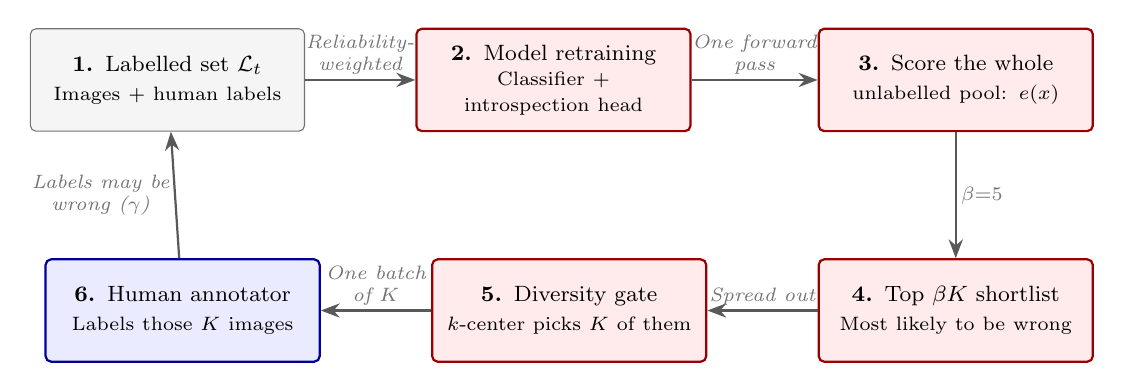
\begin{tikzpicture}[
  font=\footnotesize,
  box/.style={draw=black!55, rounded corners=2pt, align=center,
              inner sep=4pt, minimum height=13mm, text width=32mm, fill=black!4},
  newbox/.style={box, fill=red!8, draw=red!60!black, thick},
  humanbox/.style={box, fill=blue!8, draw=blue!60!black, thick},
  arr/.style={-{Stealth[length=2.4mm]}, black!65, thick},
  note/.style={font=\scriptsize\itshape, text=black!55, align=center, inner sep=1.5pt},
]
\node[box]                      (A) {\textbf{1.} Labelled set $\mathcal{L}_t$\\[1pt]
                                     {\scriptsize Images $+$ human labels}};
\node[newbox, right=14mm of A]  (B) {\textbf{2.} Model retraining\\[1pt]
                                     {\scriptsize Classifier $+$\\ introspection head}};
\node[newbox, right=16mm of B]  (C) {\textbf{3.} Score the whole\\[1pt]
                                     {\scriptsize unlabelled pool: $e(x)$}};
\node[newbox, below=16mm of C]  (D) {\textbf{4.} Top $\beta K$ shortlist\\[1pt]
                                     {\scriptsize Most likely to be wrong}};
\node[newbox, left=14mm of D]   (E) {\textbf{5.} Diversity gate\\[1pt]
                                     {\scriptsize $k$-center picks $K$ of them}};
\node[humanbox, left=14mm of E] (F) {\textbf{6.} Human annotator\\[1pt]
                                     {\scriptsize Labels those $K$ images}};
\draw[arr] (A) -- node[note, above]{Reliability-\\weighted} (B);
\draw[arr] (B) -- node[note, above]{One forward\\pass} (C);
\draw[arr] (C) -- node[note, right]{$\beta{=}5$} (D);
\draw[arr] (D) -- node[note, above]{Spread out} (E);
\draw[arr] (E) -- node[note, above]{One batch\\of $K$} (F);
\draw[arr] (F) -- node[note, left]{Labels may be\\wrong ($\gamma$)} (A);
\end{tikzpicture}

\vspace{5mm}
{\small\textbf{(b) The only change in the architecture.}}\\[2mm]
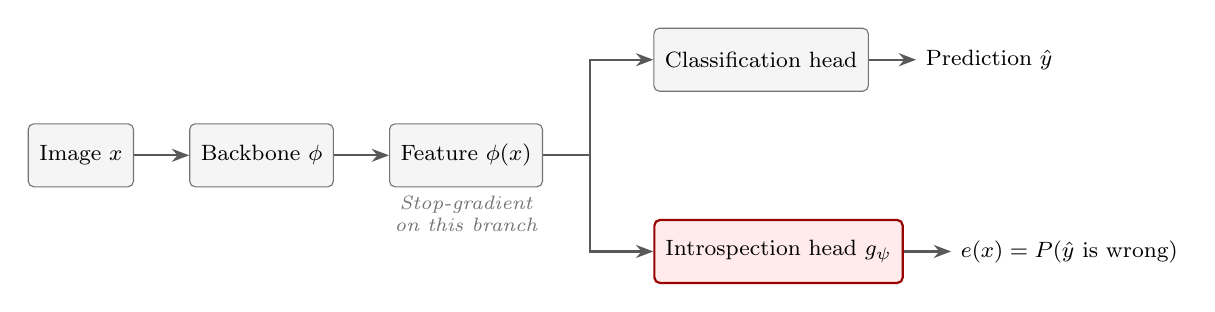
\begin{tikzpicture}[
  font=\footnotesize,
  box/.style={draw=black!55, rounded corners=2pt, align=center,
              inner sep=4pt, minimum height=8mm, fill=black!4},
  newbox/.style={box, fill=red!8, draw=red!60!black, thick},
  arr/.style={-{Stealth[length=2.2mm]}, black!65, thick},
  note/.style={font=\scriptsize\itshape, text=black!55, align=center, inner sep=1.5pt},
]
\node[box]                        (x)  {Image $x$};
\node[box, right=7mm of x]        (bb) {Backbone $\phi$};
\node[box, right=7mm of bb]       (ft) {Feature $\phi(x)$};
\node[box, above right=4mm and 14mm of ft]    (cls) {Classification head};
\node[newbox, below right=4mm and 14mm of ft] (ins) {Introspection head $g_\psi$};
\node[right=6mm of cls]  (pred) {Prediction $\hat{y}$};
\node[right=6mm of ins]  (esc)  {$e(x)=P(\hat{y}$ is wrong$)$};
\draw[arr] (x) -- (bb);
\draw[arr] (bb) -- (ft);
\draw[arr] (ft.east) -- ++(6mm,0) |- (cls.west);
\draw[arr] (ft.east) -- ++(6mm,0) |- (ins.west);
\node[note, below=0.5mm of ft] {Stop-gradient\\on this branch};
\draw[arr] (cls) -- (pred);
\draw[arr] (ins) -- (esc);
\end{tikzpicture}
\caption{Overview of \method{}. \textbf{(a)}~An active learning round:
the three red boxes represent \method{} components, the blue box is the
human annotator, and the rest constitutes the standard AL cycle.
\textbf{(b)}~Architecture: a second head consumes the classifier's
features and predicts whether the classifier is about to make an error;
because of the stop-gradient operation, this auxiliary objective does
not alter the training of the classifier itself.}
\label{fig:flow}
\end{figure}

Before the equations of Section~\ref{sec:method}, the method is
described here in plain terms; Figure~\ref{fig:flow} is a flow chart of
the same process.

\paragraph{The problem in a nutshell.} From a vast, unlabelled pool, we
can purchase human labels for only a few thousand images --- and even
the human annotator occasionally makes mistakes --- while the system
itself must decide, at each step, which images to present for
labelling.

\paragraph{Three questions per annotation cycle; conventional active
learning addresses only the first.}
\begin{enumerate}
  \item \emph{On which images is the model more likely to make
  mistakes?} Standard AL computes a hand-derived formula on the output
  probabilities (entropy, or BALD's mutual information). \method{}
  instead \emph{asks a small auxiliary head --- one that has learned
  from the model's own past mistakes --- what an error looks like}.
  \item \emph{Which of them should go together in the same batch?}
  Standard top-$K$ methods select $K$ items that are typically
  near-duplicates of one another. \method{} first generates a shortlist
  and then distributes the selected items across the feature space.
  \item \emph{To what extent should the returned labels be trusted?}
  Conventional AL trusts them completely. \method{} reduces the weight
  of those that behave like mislabelled examples during training.
\end{enumerate}

\paragraph{One round, step by step.} The numbers correspond to
Figure~\ref{fig:flow}(a).
\begin{enumerate}
  \item \textbf{Start with what is already labelled.} Hundreds of
  images, complete with labels provided by people --- some of which are
  incorrect, though we do not know which ones.
  \item \textbf{Retrain the model on them.} Two things are trained
  simultaneously: the ordinary classifier and the introspection head,
  which predicts \emph{whether the classifier is about to make a
  mistake}. Training is \emph{reliability-weighted}: images that
  persistently show a high loss are assigned less weight, as they
  behave like mislabelled samples.
  \item \textbf{Score the entire unlabelled pool} with the
  introspection head. This involves a single standard forward pass ---
  the score comes from the same network used for prediction, so there
  is no additional cost beyond the pool sweep any AL method must
  perform.
  \item \textbf{Shortlist.} The $\beta K$ images with the highest
  predicted error probabilities are retained ($\beta=5$; that is, a
  batch of 500 images is formed from a list of 2,500).
  \item \textbf{Diversity gate.} From that list, $K$ images are
  selected that are as far apart as possible --- from each other and
  from everything already labelled. This prevents the batch from
  becoming 500 copies of the same error.
  \item \textbf{Only that $K$ is sent to the person.} The labels come
  back, possibly with some errors, and the cycle begins again.
\end{enumerate}

\paragraph{What exactly is an introspection head?} Consider a student
who, while writing exam answers, also learns to identify which of their
own answers are likely to be incorrect. Softmax entropy assesses
confidence merely by observing the model's degree of uncertainty
regarding a specific query. In contrast, the introspection head
analyses the image's \emph{internal representation} and is trained on
the model's history of actual errors; consequently, it can pinpoint
regions in the feature space where the model consistently fails ---
including instances where the model is \emph{confidently} wrong, a
scenario that entropy fails to capture. Crucially, it is trained using
a stop-gradient mechanism (Figure~\ref{fig:flow}(b)): it observes the
classifier but never alters it, ensuring that its integration does not
compromise the classifier's performance.

\paragraph{Why diversity is needed in the batch.} Suppose the model
cannot distinguish between shirts and coats. Then the 500 images with
the highest scores might all be shirts. You pay for 500 labels but gain
only a single insight. The $k$-center step acquires 500 \emph{distinct}
insights instead of 500 copies of the same one; our ablation studies
show that this factor makes the single largest contribution when the
annotator is reliable.

\paragraph{Why returned labels are not blindly trusted.} Deep networks
learn the clean, consistent parts of a dataset before memorising the
corrupted ones. Thus, samples that consistently exhibit a high loss
across epochs are disproportionately likely to have incorrect labels.
\method{} down-weights these samples (to $0.1$) rather than discarding
them, allowing genuinely difficult-yet-correct examples to persist.
This reasoning relies on a crucial prerequisite: for ``high loss'' to
imply ``likely mislabelled'', the model must already be sufficiently
proficient; otherwise, a high loss simply indicates that the sample
``has not yet been learned'' --- and Section~\ref{sec:results}
demonstrates exactly where this assumption fails.

\paragraph{Cost.} A two-layer MLP. Because its size is fixed
($d\to128\to1$) while the backbone's is not, its relative cost falls as
the model grows: \FmnistHeadPct\% of the small CNN used here,
\CifarHeadPct\% of a ResNet-18, and less again on anything larger. No
additional forward pass during querying, and no change to the
classifier's gradients. Any model trained using the standard
classification pipeline can adopt this.

\begin{table}[pos=t]
\centering\small
\caption{The three components, the failure each prevents, and the test
that verifies them individually.}
\label{tab:components}
\begin{tabular}{R{0.21}R{0.29}R{0.22}R{0.16}}
\toprule
Component & Failure prevented & How it works & Verification test \\
\midrule
Introspection head & Hand-crafted uncertainty is mis-calibrated and
ignores the model's error history & Learned $P(\text{error})$ from
detached features & AUROC analysis (Figure~\ref{fig:auroc}) \\
Diversity gate & Top-$K$ batch of near-duplicates based on point-wise
scores & $k$-center on the top $\beta K$, seeded with the labelled set
& Ablation \emph{without diversity} \\
Reliability weighting & Training that treats incorrect human labels as
correct & Low-loss EMA weight decay & Ablation \emph{without
reliability} \\
\bottomrule
\end{tabular}
\end{table}

\section{Method}\label{sec:method}
\subsection{Setting}
Pool-based batch active learning with an imperfect oracle. Let
$\mathcal{U}=\{x_i\}$ be the unlabelled pool and $\mathcal{L}_t$ the
labelled set at round $t$, where $|\mathcal{L}_0|=n_0$. In each round
the learner selects a batch $Q_t\subset\mathcal{U}$ of size $K$; the
human oracle returns $\tilde{y}=y$ with probability $1-\gamma$ and an
incorrect class chosen uniformly at random with probability $\gamma$
(symmetric noise; $\gamma=0$ corresponds to the standard perfect
oracle). After each round, the model $f_\theta$ is retrained from
scratch on $\mathcal{L}_{t+1}=\mathcal{L}_t\cup Q_t$, and test accuracy
is reported as a function of $|\mathcal{L}_t|$.

\subsection{Introspection head}\label{sec:head}
Let $\phi(x)\in\mathbb{R}^d$ be the penultimate feature from the
backbone and $f_\theta(x)=W\,\mathrm{drop}(\phi(x))$ the class logit.
We introduce $g_\psi:\mathbb{R}^d\to\mathbb{R}$, a two-layer MLP
($d\to128\to1$) that computes the \emph{introspection score}
\begin{equation}
  e(x)=\sigma\!\big(g_\psi(\mathrm{sg}[\phi(x)])\big)\in(0,1),
\end{equation}
where $\mathrm{sg}[\cdot]$ denotes the stop-gradient operation: the
auxiliary loss never interferes with the backbone, ensuring that the
classifier's training dynamics remain identical across all methods. The
training target is the model's \emph{own current error indicator}
$z=\mathbb{1}[\arg\max f_\theta(x)\neq\tilde{y}]$, computed on the fly
for each mini-batch, using class-balanced BCE,
\begin{equation}
  \mathcal{L}_{\mathrm{aux}}
  =\mathrm{BCE}_{\omega}\big(g_\psi(\mathrm{sg}[\phi(x)]),\,z\big),\qquad
  \omega=\mathrm{clip}\!\Big(\tfrac{1-\hat{\pi}}{\hat{\pi}},1,20\Big),
\end{equation}
where $\hat{\pi}$ is a running estimate of the error rate ($\omega$
re-balances the positive class, which vanishes as training converges).
Errors are frequent early in training, allowing the head to learn which
regions of the feature space are difficult for the classifier; since
the input consists of features rather than logits, the score does not
depend on any transformation of softmax confidence. By estimating a
\emph{bounded probability} instead of an unbounded loss value
\citep{yoo2019}, the scale-variation issue --- which typically
necessitates loss-ranking techniques in Learning-Loss approaches --- is
entirely avoided.

\subsection{Diversity gate}\label{sec:gate}
Selecting the top $K$ samples by $e(x)$ leads to batch redundancy, as
nearby neighbours tend to have similar scores. Instead, \method{}
selects the top $\beta K$ candidates ($\beta=5$) by introspection score
and then performs greedy $k$-center selection \citep{sener2018} on
these candidates in feature space --- \emph{seeded with the features of
the currently labelled set}: each of the $K$ selections maximises the
minimum distance to all labelled points and to previously selected
samples. Consequently, the batch is simultaneously (i) concentrated in
regions where the model is expected to fail, and (ii) spread out in
feature space, away from already annotated regions.

\subsection{Reliability-weighted label acceptance}\label{sec:rel}
Labels obtained from noisy annotators can do more harm than good.
During retraining, \method{} maintains an EMA of the loss for each
labelled sample, $\bar{\ell}_i\leftarrow0.7\,\bar{\ell}_i+0.3\,\ell_i$,
and applies the small-loss criterion \citep{han2018} after an initial
phase of $\max(3,E/5)$ epochs: within each mini-batch, the fraction
$(1-\gamma)$ of samples with the lowest EMA loss are assigned a weight
of $1$ while the rest receive $0.1$, and the classification loss is
computed as a weighted average. Since deep networks learn clean labels
before corrupted ones, samples with a consistently high loss are
disproportionately likely to carry corrupted annotations;
down-weighting rather than discarding them preserves information from
clean yet difficult examples. Following co-teaching \citep{han2018}, we
assume $\gamma$ is known; estimating it online is a separate,
established problem.

\begin{algorithm}[t]
\caption{\method{}: one active learning round}
\begin{algorithmic}[1]
\State Train $(\theta, \psi)$ on $\mathcal{L}_t$: weighted CE
(Section~\ref{sec:rel}) $+$ class-balanced BCE
for $g_\psi$ on $\mathrm{sg}[\phi(x)]$ (Section~\ref{sec:head})
\State For all $x_i\in\mathcal{U}$, $e_i\gets\sigma(g_\psi(\phi(x_i)))$
\State $C\gets$ top $\beta K$ of $\mathcal{U}$ by $e_i$
\State $Q_t\gets$ greedy $k$-center on $\{\phi(x):x\in C\}$, seeded with
$\{\phi(x):x\in\mathcal{L}_t\}$
\State $\mathcal{L}_{t+1}\gets\mathcal{L}_t\cup\{(x,\tilde{y}(x)):x\in Q_t\}$
\Comment{$\tilde{y}$: noisy human oracle}
\end{algorithmic}
\end{algorithm}

\section{Application: annotation that runs with almost no intervention}
\label{sec:application}
The approach described in Section~\ref{sec:method} is effective only
when integrated into a workflow that a busy expert is willing to
tolerate. This section describes the intended application scenario ---
where a person simply labels the items presented to them without
performing any other task --- and clarifies which decisions \method{}
removes from the human's hands and which remain.

\paragraph{Context: a routine expert-labelling task.} Consider a
haematology laboratory performing white blood cell differential counts.
A digital microscope continuously generates images of individual cells;
a trained morphologist classifies them as part of their daily routine.
The pool of unlabelled cells is effectively infinite, expert time is
the only scarce resource, and expert labels are good but imperfect:
rare and immature forms are genuinely ambiguous, and inter-observer
disagreement on such cells is comparable to evaluator disagreement on
wildlife tracks \citep{petso2026} or annotation errors in benchmark
corpora \citep{hussain2026}. Our BloodMNIST experiment
(Section~\ref{sec:results}) is an open, reproducible proxy for this
exact scenario: eight classes of white blood cells, a capable baseline
model, and a limited budget.

\paragraph{What ``minimal intervention'' actually entails.} The
annotator's entire involvement consists of opening the worklist,
viewing images of $K$ cells, pressing one of eight class buttons for
each, and closing the worklist. There is no pool to browse, no sorting
to perform, no thresholds to set, no model outputs to verify, and no
need to express uncertainty or explain decisions. Everything else ---
determining which cells warrant expert attention, ensuring the worklist
does not contain $K$ variants of the same cell, and assessing the
impact of each returned label on the model --- happens inside the
classifier. Table~\ref{tab:burden} compares how this same cycle is
executed in the applied literature and under \method{}.

\begin{table}[pos=t]
\centering\small
\caption{Where the labour goes in the expert-annotation cycle. Left
column: current practice in applied HITL systems, such as the pooled
ranking by three evaluators of \citet{petso2026}; right column: the
same cycle under \method{}.}
\label{tab:burden}
\begin{tabular}{@{}R{0.20}R{0.37}R{0.35}@{}}
\toprule
Aspect & Conventional expert curation & \method{} \\
\midrule
Selection scope & Expert manually browses or sorts the pool &
Introspection head sorts the pool; the expert receives a worklist \\
Batch composition & Unspecified; top-scoring samples are often
duplicates & $k$-center gate ensures a diverse worklist \\
Selection rule & Heuristic selection and per-dataset tuning (entropy,
margin, \ldots) & Learned from the model's own errors; no threshold
setting required \\
Annotator errors & Dual annotation and adjudication meetings &
Low-loss weighting absorbs errors; no re-labelling phase needed \\
Model monitoring & Expert verifies predictions to decide when to
intervene & Automated capability check each round (below) \\
Interface & Custom-built active learning tooling \citep{piccoli2026} &
Standard labelling interface, $K$ samples per session\\
\bottomrule
\end{tabular}
\end{table}

\paragraph{Each component addresses an error and also reduces human
labour.} The introspection head replaces the manual sample selection
process --- which, in systems such as that of \citet{petso2026},
consumes the lion's share of an expert's time --- and does so without
requiring additional model maintenance; the score is derived from the
same forward pass used for prediction. The diversity gate prevents
wasted effort on labelling repetitive samples, the most common way
annotation budgets are squandered, without the expert even needing to
notice the repetition. The reliability gate eliminates the adjudication
step: since the learner itself absorbs the burden of error-prone
labels, there is no need to label each image twice, nor must the
annotator communicate their uncertainty. The cycle is asynchronous ---
labels return when convenient, and retraining occurs between sessions
--- so the expert is never held up by the model, nor the model by the
expert.

\paragraph{What the manager still needs to determine.} Three
parameters, each set once. (i)~The batch size $K$, which depends on how
many images an annotator can comfortably label in a single session.
(ii)~A working estimate of the annotator error rate $\gamma$ for use in
the reliability gate; following co-teaching \citep{han2018}, we treat
this as known, and in a laboratory setting it can be derived from a
small doubly annotated pilot sample. (iii)~A \emph{capability gate}:
our results indicate that introspection-based selection and reliability
weighting should be activated only after the base model has become
sufficiently proficient --- the rule of thumb is to spend the initial
portion of the budget on random sampling and to activate \method{} only
once the epoch-wise test accuracy, or the validation AUROC of the
introspection head, crosses a threshold. For the two datasets where the
model is capable from the very first round, this gate is passed
immediately; for CIFAR-10 trained from scratch, the threshold is never
met within the given budget --- which is why \method{} should not be
used in that case (Section~\ref{sec:results}).

\paragraph{Implementation checklist.} (1)~Train the existing classifier
with an auxiliary head; no further changes to the training code.
(2)~Check round-0 accuracy against the capability gate; if it fails,
label the initial subset at random. (3)~In each round, score the pool,
create a shortlist, apply the $k$-center gate, and send $K$ images to
the annotation tool. (4)~Accept returned labels with reliability
weighting enabled only if $\gamma > 0$. (5)~Log the introspection AUROC
for each round; a drop in this AUROC signals a reversion to random
selection.

\paragraph{Also outside the laboratory.} The same mould --- an infinite
pool, a scarce expert, a pre-built one-click labelling interface, and a
tolerable level of annotator error --- describes wildlife footprint
curation \citep{petso2026}, whole-slide image patch review
\citep{lou2026}, moderation and fake-news sorting \citep{comito2026},
and industrial vision-based inspection. In all of them, the human's
work under \method{} remains what it already was: seeing a picture,
saying its name, moving to the next one.

\section{Experimental design}\label{sec:experiments}

\subsection{Datasets}\label{sec:datasets}
Three public image benchmarks, summarised in
Table~\ref{tab:datasets}, span the range of base-model capability on
which the logic of the method depends. All three are standard,
openly redistributable and small enough that the full grid of
experiments can be repeated on a single GPU, which matters for a
claim that rests on the \emph{boundary} between two regimes rather
than on a single headline number.

\emph{Fashion-MNIST} \citep{xiao2017} contains $28\times28$ grayscale
photographs of clothing articles from a catalogue, in ten classes
(t-shirt, trouser, pullover, dress, coat, sandal, shirt, sneaker, bag,
ankle boot), split into 60,000 training and 10,000 test images. It was
designed as a drop-in replacement for MNIST that is genuinely harder,
and it suits us for two reasons. First, a small CNN reaches roughly
74\% accuracy from only a few hundred labels, so the base model is
already competent when selection begins --- exactly the regime in
which the introspection head is supposed to have something to say.
Second, several of its classes (shirt, coat, pullover) are confusable
in a structured way, so a selection method that keeps picking the same
confusion is visibly punished, which is what makes the diversity gate
measurable.

\emph{BloodMNIST} is the peripheral blood cell subset of MedMNIST~v2
\citep{yang2023}, derived from the microscopy collection of
\citet{acevedo2020}: single-cell images of individual normal blood
cells from patients without infection or oncological disease, captured
in a clinical laboratory and labelled by expert pathologists into eight
classes (basophil, eosinophil, erythroblast, immature granulocyte,
lymphocyte, monocyte, neutrophil, platelet). MedMNIST~v2 centre-crops
and resamples them to $28\times28$ RGB and supplies a fixed split of
11,959 training and 3,421 test images. We include it for three
reasons. It is a genuine medical imaging task, so it instantiates the
expert-annotation workflow of Section~\ref{sec:application} rather than
merely alluding to it; its eight classes are markedly imbalanced, which
is the normal condition of clinical data and a harder test of batch
construction than a uniform benchmark; and, because it shares the input
resolution of Fashion-MNIST, it can reuse that dataset's backbone and
training recipe without a single retuned hyperparameter. That last
point is what turns it into an out-of-the-box transfer test rather than
a curated demonstration.

\emph{CIFAR-10} \citep{krizhevsky2009} contains $32\times32$ colour
photographs of natural objects in ten classes, split into 50,000
training and 10,000 test images. Paired with a ResNet-18
\citep{he2016} trained from scratch, it is included deliberately as the
hard case: at these budget sizes the network reaches only around 46\%
accuracy before selection begins, so every informativeness signal
computed from it --- ours included --- is estimated from a model that
does not yet know much. It is the dataset on which we expect, and
find, the method to fail, and it is what allows the paper to state a
condition of use instead of an unqualified claim.

\begin{table}[pos=t]
\centering\small
\caption{The three datasets, what they contain, and the regime each one
probes. ``Round-0 accuracy'' is the mean test accuracy of the model
trained on the initial random seed set --- the state before any
selection strategy has had an effect --- and serves as the practical
proxy for the capability gate of Section~\ref{sec:application}.}
\label{tab:datasets}
\begin{tabular}{@{}R{0.155}R{0.30}cc R{0.19}@{}}
\toprule
Dataset & Content and source & Classes & Train / test &
Regime probed \\
\midrule
Fashion-MNIST &
Grayscale $28\times28$ catalogue photographs of clothing articles;
several structurally confusable classes \citep{xiao2017} &
10 & 60,000 / 10,000 &
Capable base model (round-0 ${\sim}\FmnistRoundZero\%$) \\[3pt]
BloodMNIST &
Single-cell peripheral blood microscopy, expert-labelled, imbalanced
classes; $28\times28$ RGB, MedMNIST~v2 subset
\citep{yang2023,acevedo2020} &
8 & 11,959 / 3,421 &
Capable base model (round-0 ${\sim}\BloodRoundZero\%$); application-realistic \\[3pt]
CIFAR-10 &
Colour $32\times32$ photographs of natural objects; ResNet-18 trained
from scratch \citep{krizhevsky2009,he2016} &
10 & 50,000 / 10,000 &
Cold start (round-0 ${\sim}\CifarRoundZero\%$) \\
\bottomrule
\end{tabular}
\end{table}

\subsection{Protocol}
\textbf{Backbones and annotation schedule.} Fashion-MNIST and
BloodMNIST use the same four-layer convolutional CNN (penultimate
dimension $d{=}256$), starting from $n_0{=}500$ labels and acquiring
$K{=}500$ per round for 5 rounds. CIFAR-10 uses a CIFAR-adapted
ResNet-18 ($3{\times}3$ stem, no max-pooling, $d{=}512$), starting from
$n_0{=}1{,}000$ and acquiring $K{=}1{,}000$ per round for 5 rounds.
Dropout ($p{=}0.25$) before the final layer serves a dual purpose:
regularisation, and MC-dropout for BALD. \textbf{Training.} SGD
(momentum $0.9$, weight decay $5\times10^{-4}$), cosine schedule;
Fashion-MNIST and BloodMNIST: 30 epochs, batch size 64, lr $0.02$;
CIFAR-10: 30 epochs, batch size 128, lr $0.05$; standard crop and flip
augmentation; retraining from scratch in each round. No hyperparameters
were retuned for BloodMNIST --- it inherits the Fashion-MNIST protocol
exactly, so its results represent a genuine as-is transfer rather than
a curated demonstration.

\textbf{Oracle.} Noise-free ($\gamma{=}0$) and noisy ($\gamma{=}0.2$
symmetric); the initial seed set is labelled by the same oracle. Test
set labels are never corrupted. \textbf{Baselines.} Random, Entropy,
BALD (10 MC-dropout passes) \citep{gal2017}, Core-set $k$-center
\citep{sener2018}, Learning-Loss \citep{yoo2019} --- the prior learned
acquisition signal, reimplemented with its pairwise ranking objective
and without detachment, so its gradients reach the backbone as in the
original --- and BADGE \citep{ash2020}, $k$-means++ seeding on
hypothetical gradient embeddings. To separate the two halves of our
method we also run \emph{BADGE $+$ reliability}: BADGE acquisition with
our label-acceptance gate, which isolates the gate from the selector it
was designed alongside. All methods use identical backbones, optimisers,
schedules and seeds; the introspection head is present in every run,
though unused for selection, to keep parameter counts and RNG streams
matched. \textbf{Ablations}, on all three datasets:
\method{} without the diversity gate (top-$K$ introspection only) under
the perfect oracle, and \method{} without the reliability weight under
the noisy one. We run them on CIFAR-10 as well as on the two
inexpensive datasets specifically so that the cold-start failure can be
attributed to a component rather than guessed at. \textbf{Metrics.} Test accuracy after each round; final
accuracy; and area under the accuracy--budget curve (AUBC,
trapezoidal, normalised by the budget range). We report mean $\pm$
standard deviation over \FmnistNoisyNSeeds{} seeds for Fashion-MNIST
and BloodMNIST and \CifarNoisyNSeeds{} seeds for the computationally
expensive CIFAR-10 grid, together with a paired $t$-test on matched
seeds wherever \method{} is compared against the strongest baseline
(same seed $\Rightarrow$ same initial labelled set). Error-prediction
quality is assessed separately, by the AUROC of the introspection score
and of softmax entropy against the model's actual test-set errors.

\section{Results}\label{sec:results}

\begin{table}[pos=t]
\centering\small
\caption{Final accuracy and AUBC (mean $\pm$ standard deviation across
seeds, \%; \FmnistNoisyNSeeds{} seeds for Fashion-MNIST and BloodMNIST,
\CifarNoisyNSeeds{} for CIFAR-10). The best AUBC in each scenario is in
bold; final accuracy is discussed separately because the two metrics
yield different conclusions on BloodMNIST. Generated automatically from
\texttt{results/results.csv}.}
\label{tab:main}
\IfFileExists{../results/summary_table.tex}{\begin{tabular}{llcc}
\toprule
Setting & Method & Final acc. (\%) & AUBC (\%) \\
\midrule
Fashion-MNIST, clean & Random & 86.28 $\pm$ 0.41 & 82.08 $\pm$ 0.22 \\
Fashion-MNIST, clean & Entropy & 87.11 $\pm$ 0.48 & 82.80 $\pm$ 0.33 \\
Fashion-MNIST, clean & BALD & 88.03 $\pm$ 0.70 & 82.57 $\pm$ 0.68 \\
Fashion-MNIST, clean & Coreset & 83.86 $\pm$ 0.48 & 80.95 $\pm$ 0.35 \\
Fashion-MNIST, clean & Learning-Loss & 86.03 $\pm$ 0.94 & 82.03 $\pm$ 0.29 \\
Fashion-MNIST, clean & BADGE & \textbf{88.87 $\pm$ 0.22} & \textbf{84.77 $\pm$ 0.24} \\
Fashion-MNIST, clean & IRIS (ours) & 87.61 $\pm$ 0.65 & 82.65 $\pm$ 0.52 \\
Fashion-MNIST, clean & IRIS-grad (ours) & 87.41 $\pm$ 0.50 & 82.73 $\pm$ 0.68 \\
Fashion-MNIST, clean & IRIS w/o  diversity & 86.31 $\pm$ 0.74 & 81.32 $\pm$ 0.88 \\
\midrule
Fashion-MNIST, noisy $\gamma{=}0.2$ & Random & 83.71 $\pm$ 0.54 & 79.61 $\pm$ 0.39 \\
Fashion-MNIST, noisy $\gamma{=}0.2$ & Entropy & 84.30 $\pm$ 0.47 & 79.20 $\pm$ 0.91 \\
Fashion-MNIST, noisy $\gamma{=}0.2$ & BALD & 81.92 $\pm$ 1.30 & 77.81 $\pm$ 0.46 \\
Fashion-MNIST, noisy $\gamma{=}0.2$ & Coreset & 81.89 $\pm$ 0.46 & 78.39 $\pm$ 0.46 \\
Fashion-MNIST, noisy $\gamma{=}0.2$ & Learning-Loss & 83.27 $\pm$ 1.00 & 77.79 $\pm$ 0.83 \\
Fashion-MNIST, noisy $\gamma{=}0.2$ & BADGE & 86.59 $\pm$ 0.30 & 81.72 $\pm$ 0.20 \\
Fashion-MNIST, noisy $\gamma{=}0.2$ & BADGE + reliability & \textbf{87.52 $\pm$ 0.40} & \textbf{82.83 $\pm$ 0.24} \\
Fashion-MNIST, noisy $\gamma{=}0.2$ & IRIS (ours) & 85.68 $\pm$ 0.61 & 80.40 $\pm$ 0.38 \\
Fashion-MNIST, noisy $\gamma{=}0.2$ & IRIS-grad (ours) & 84.95 $\pm$ 0.95 & 80.25 $\pm$ 0.57 \\
Fashion-MNIST, noisy $\gamma{=}0.2$ & IRIS w/o  reliability & 84.55 $\pm$ 0.25 & 79.28 $\pm$ 0.48 \\
\midrule
BloodMNIST, clean & Random & 89.47 $\pm$ 0.68 & 83.63 $\pm$ 0.98 \\
BloodMNIST, clean & Entropy & 91.25 $\pm$ 0.97 & 82.10 $\pm$ 1.33 \\
BloodMNIST, clean & BALD & 91.51 $\pm$ 0.73 & 83.94 $\pm$ 0.84 \\
BloodMNIST, clean & Coreset & 85.83 $\pm$ 1.27 & 82.10 $\pm$ 0.80 \\
BloodMNIST, clean & Learning-Loss & 88.15 $\pm$ 1.89 & 75.71 $\pm$ 1.56 \\
BloodMNIST, clean & BADGE & \textbf{92.20 $\pm$ 0.94} & \textbf{85.10 $\pm$ 0.43} \\
BloodMNIST, clean & IRIS (ours) & 90.62 $\pm$ 0.91 & 81.14 $\pm$ 0.53 \\
BloodMNIST, clean & IRIS-grad (ours) & 90.61 $\pm$ 0.97 & 80.28 $\pm$ 0.76 \\
BloodMNIST, clean & IRIS w/o  diversity & 87.67 $\pm$ 1.73 & 79.27 $\pm$ 0.95 \\
\midrule
BloodMNIST, noisy $\gamma{=}0.2$ & Random & 86.94 $\pm$ 0.75 & 80.00 $\pm$ 0.98 \\
BloodMNIST, noisy $\gamma{=}0.2$ & Entropy & 86.52 $\pm$ 1.69 & 76.68 $\pm$ 1.34 \\
BloodMNIST, noisy $\gamma{=}0.2$ & BALD & 83.32 $\pm$ 1.08 & 75.25 $\pm$ 1.47 \\
BloodMNIST, noisy $\gamma{=}0.2$ & Coreset & 87.09 $\pm$ 0.45 & 78.97 $\pm$ 1.08 \\
BloodMNIST, noisy $\gamma{=}0.2$ & Learning-Loss & 80.53 $\pm$ 2.44 & 70.75 $\pm$ 1.73 \\
BloodMNIST, noisy $\gamma{=}0.2$ & BADGE & 88.42 $\pm$ 0.70 & 80.90 $\pm$ 1.20 \\
BloodMNIST, noisy $\gamma{=}0.2$ & BADGE + reliability & \textbf{89.37 $\pm$ 0.70} & \textbf{81.09 $\pm$ 1.22} \\
BloodMNIST, noisy $\gamma{=}0.2$ & IRIS (ours) & 87.82 $\pm$ 0.75 & 78.52 $\pm$ 0.77 \\
BloodMNIST, noisy $\gamma{=}0.2$ & IRIS-grad (ours) & 88.15 $\pm$ 1.48 & 78.37 $\pm$ 1.08 \\
BloodMNIST, noisy $\gamma{=}0.2$ & IRIS w/o  reliability & 87.35 $\pm$ 1.15 & 77.33 $\pm$ 0.90 \\
\midrule
CIFAR-10, clean & Random & 74.50 $\pm$ 0.46 & 61.99 $\pm$ 0.58 \\
CIFAR-10, clean & Entropy & 73.42 $\pm$ 2.41 & 58.92 $\pm$ 1.43 \\
CIFAR-10, clean & BALD & 73.71 $\pm$ 1.14 & 59.91 $\pm$ 0.53 \\
CIFAR-10, clean & Coreset & 71.43 $\pm$ 0.57 & 59.27 $\pm$ 0.51 \\
CIFAR-10, clean & Learning-Loss & 63.31 $\pm$ 4.85 & 51.03 $\pm$ 1.23 \\
CIFAR-10, clean & BADGE & \textbf{73.50 $\pm$ 3.05} & \textbf{62.47 $\pm$ 0.56} \\
CIFAR-10, clean & IRIS (ours) & 70.91 $\pm$ 1.71 & 59.26 $\pm$ 0.78 \\
CIFAR-10, clean & IRIS-grad (ours) & 71.32 $\pm$ 3.46 & 58.47 $\pm$ 1.37 \\
CIFAR-10, clean & IRIS w/o  diversity & 68.44 $\pm$ 3.15 & 56.67 $\pm$ 0.78 \\
\midrule
CIFAR-10, noisy $\gamma{=}0.2$ & Random & 63.24 $\pm$ 0.55 & 54.00 $\pm$ 0.51 \\
CIFAR-10, noisy $\gamma{=}0.2$ & Entropy & 62.16 $\pm$ 1.29 & 51.47 $\pm$ 0.83 \\
CIFAR-10, noisy $\gamma{=}0.2$ & BALD & 60.55 $\pm$ 1.42 & 49.00 $\pm$ 1.28 \\
CIFAR-10, noisy $\gamma{=}0.2$ & Coreset & 60.36 $\pm$ 0.29 & 49.89 $\pm$ 0.39 \\
CIFAR-10, noisy $\gamma{=}0.2$ & Learning-Loss & 53.97 $\pm$ 3.78 & 45.93 $\pm$ 0.99 \\
CIFAR-10, noisy $\gamma{=}0.2$ & BADGE & 63.15 $\pm$ 1.52 & 53.97 $\pm$ 0.32 \\
CIFAR-10, noisy $\gamma{=}0.2$ & BADGE + reliability & \textbf{64.59 $\pm$ 1.16} & \textbf{54.79 $\pm$ 0.28} \\
CIFAR-10, noisy $\gamma{=}0.2$ & IRIS (ours) & 62.20 $\pm$ 0.30 & 51.69 $\pm$ 1.07 \\
CIFAR-10, noisy $\gamma{=}0.2$ & IRIS-grad (ours) & 59.65 $\pm$ 1.70 & 50.68 $\pm$ 0.37 \\
CIFAR-10, noisy $\gamma{=}0.2$ & IRIS w/o  reliability & 62.09 $\pm$ 0.40 & 50.97 $\pm$ 0.53 \\
\bottomrule
\end{tabular}
}%
{\emph{[Results table pending]}}
\end{table}

\begin{figure}[pos=p]
\centering
\IfFileExists{../results/curves_fmnist_noise0.0.png}{%
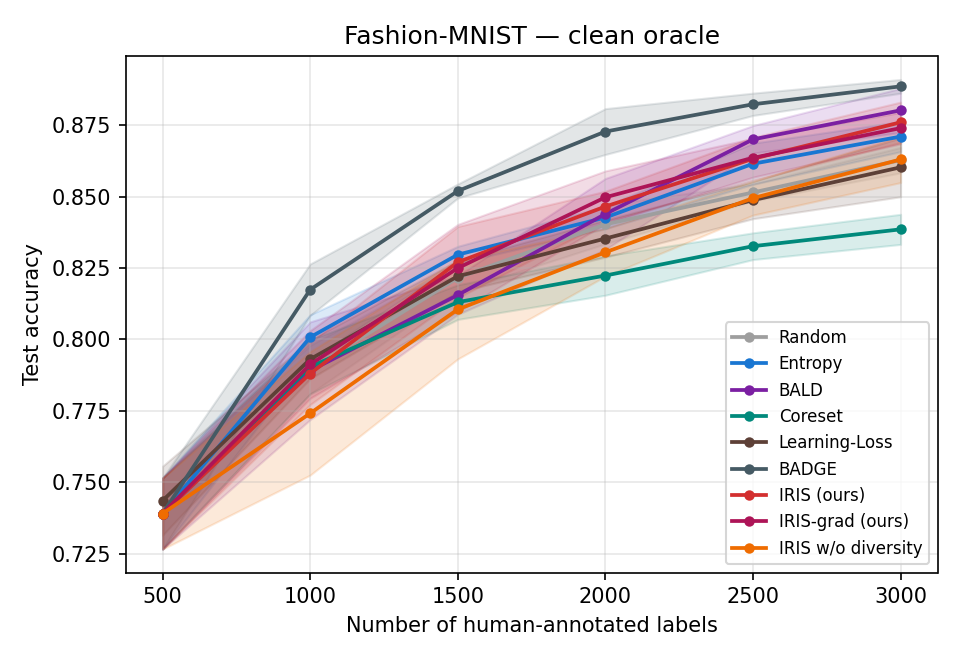
\includegraphics[width=.48\linewidth]{../results/curves_fmnist_noise0.0.png}}{}
\IfFileExists{../results/curves_fmnist_noise0.2.png}{%
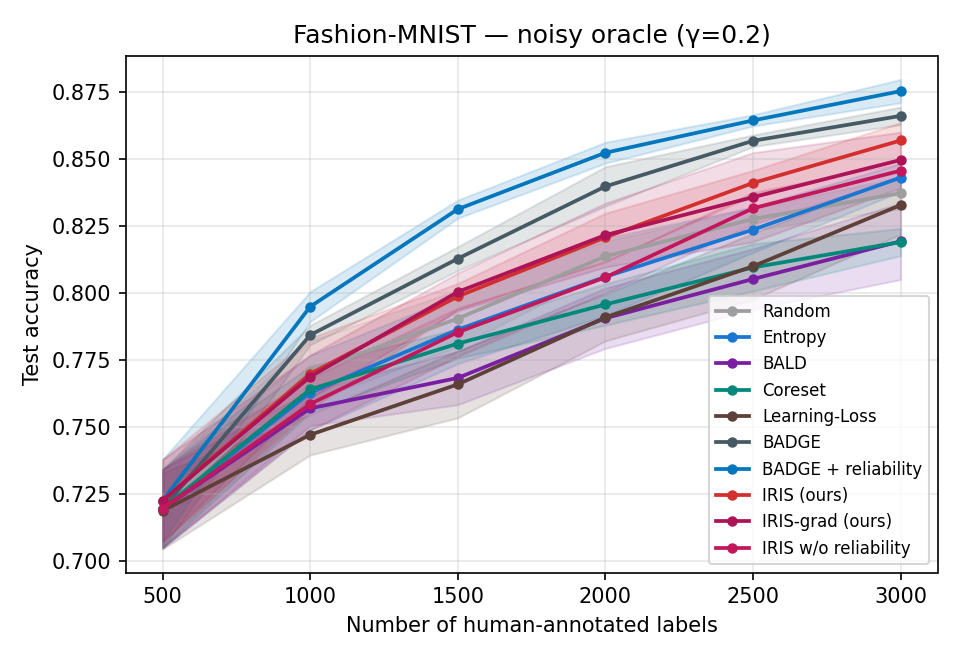
\includegraphics[width=.48\linewidth]{../results/curves_fmnist_noise0.2.png}\\}{}
\IfFileExists{../results/curves_bloodmnist_noise0.0.png}{%
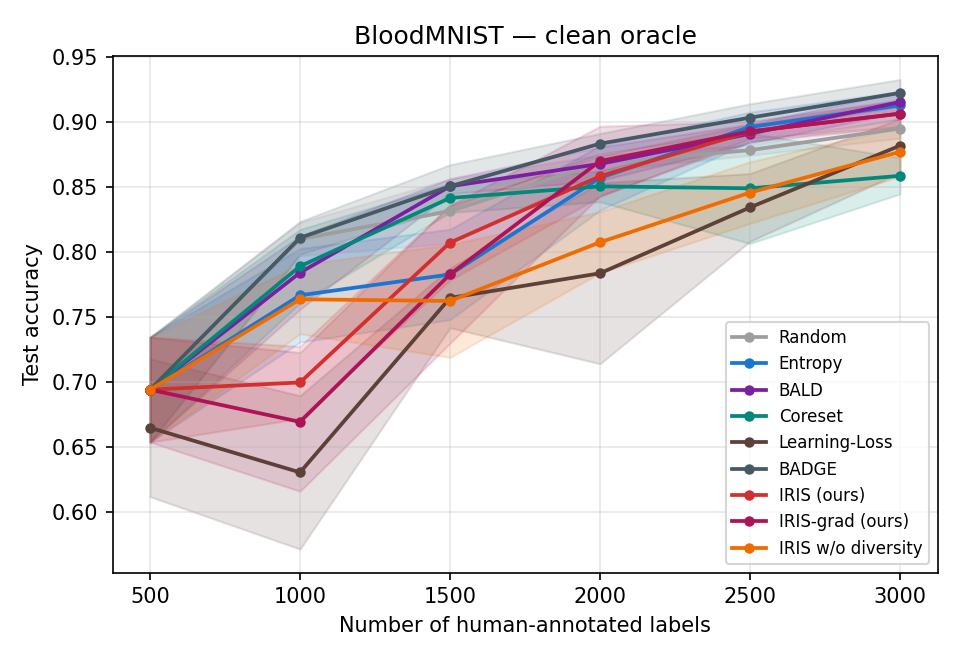
\includegraphics[width=.48\linewidth]{../results/curves_bloodmnist_noise0.0.png}}{}
\IfFileExists{../results/curves_bloodmnist_noise0.2.png}{%
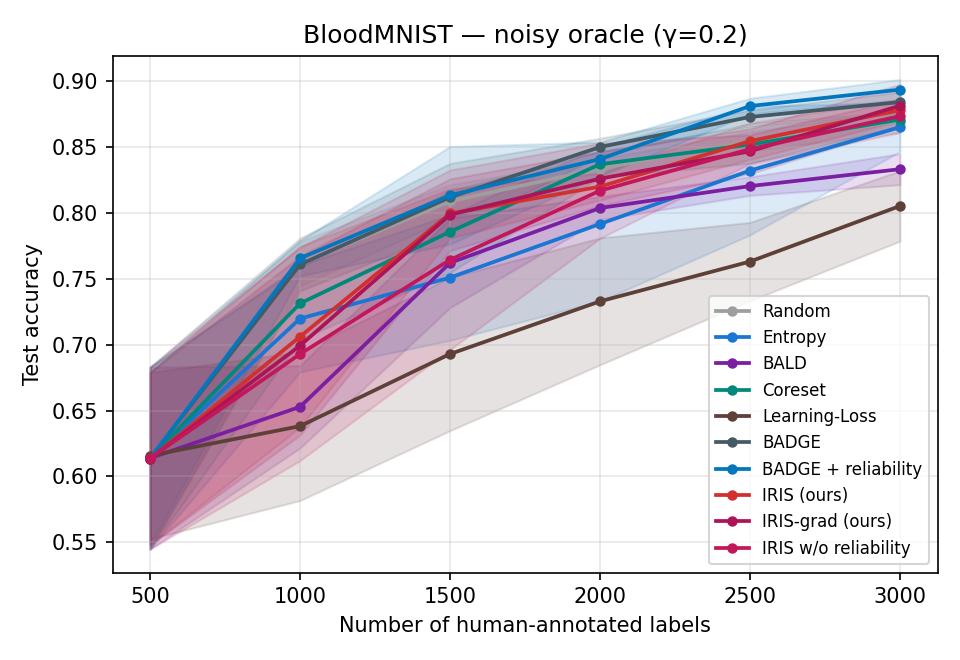
\includegraphics[width=.48\linewidth]{../results/curves_bloodmnist_noise0.2.png}\\}{}
\IfFileExists{../results/curves_cifar10_noise0.0.png}{%
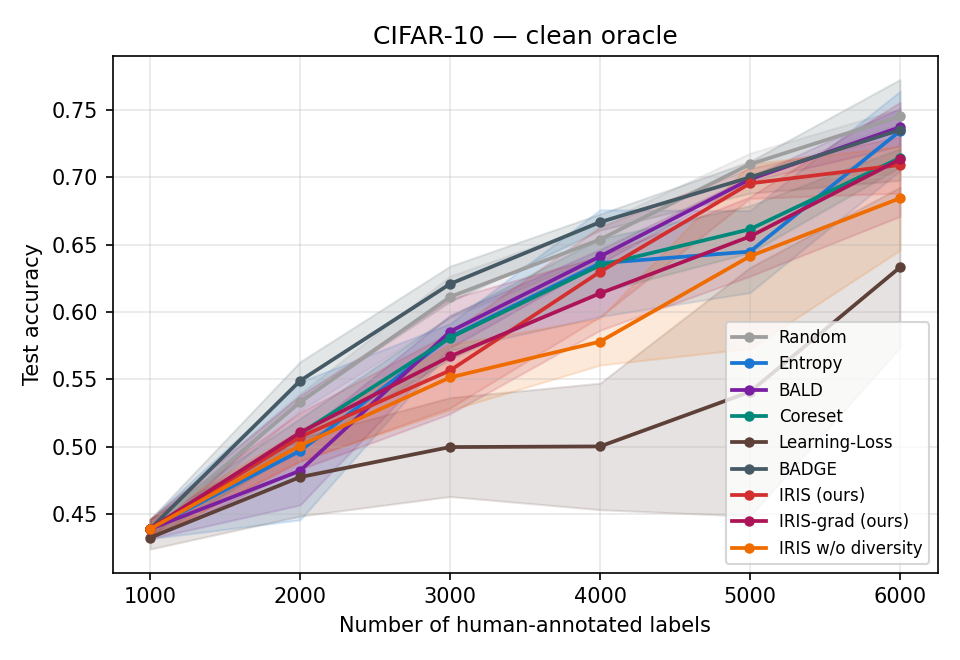
\includegraphics[width=.48\linewidth]{../results/curves_cifar10_noise0.0.png}}{}
\IfFileExists{../results/curves_cifar10_noise0.2.png}{%
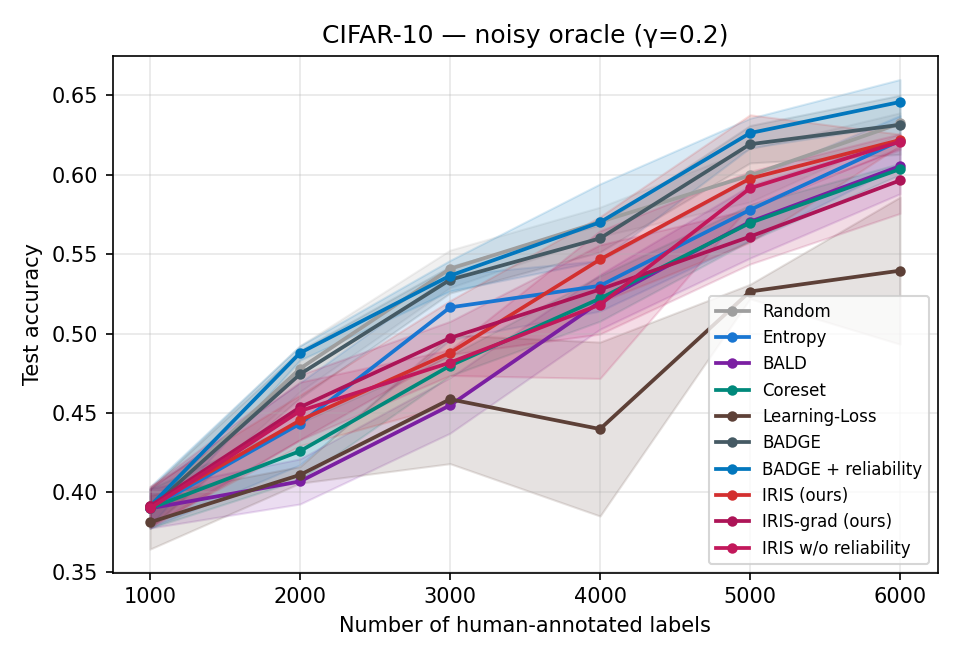
\includegraphics[width=.48\linewidth]{../results/curves_cifar10_noise0.2.png}}{}
\caption{Accuracy versus annotation budget (mean $\pm$ standard
deviation across seeds; \FmnistNoisyNSeeds{} seeds for Fashion-MNIST
and BloodMNIST, \CifarNoisyNSeeds{} seeds for CIFAR-10). Left column:
perfect oracle. Right column: noisy oracle ($\gamma{=}0.2$). Rows, top
to bottom: Fashion-MNIST, BloodMNIST, CIFAR-10 --- that is, two
scenarios with a capable model, followed by the cold start.}
\label{fig:curves}
\end{figure}

\paragraph{Three regimes.} The results separate into three regimes,
distinguished by the initial capability of the base model at the start
of selection (Table~\ref{tab:datasets}). For the two datasets where the
model is already capable --- Fashion-MNIST and BloodMNIST --- every
method carrying an informativeness signal improves on random sampling
under the noisy oracle the applied literature considers realistic, and
the ordering among them is where the interesting result lies. On
CIFAR-10, where the model starts from scratch and reaches only
${\sim}\CifarRoundZero\%$ accuracy, no \emph{acquisition} strategy
beats random sampling; only the reliability gate does. For BloodMNIST, the two
metrics disagree in an instructive manner; rather than glossing over
this discrepancy, we present it as a result in itself.

\paragraph{Which half does the work.} The comparison against
Learning-Loss and BADGE splits our own method in two, and the halves
behave differently enough that reporting a single verdict would hide
the result. As an acquisition signal, the introspection head is good
but not best. It improves on Learning-Loss --- the method that
introduced the idea of learning the selection signal --- by
\FmnistNoisyLearnlossGap{} points on Fashion-MNIST and
\BloodNoisyLearnlossGap{} on BloodMNIST under noise, which is the
comparison our design was aimed at and which it wins clearly. It also
beats Entropy, BALD, Core-set and random sampling there. But BADGE
beats \emph{it}: \FmnistNoisyBadgeFinal\% against
\FmnistNoisyIrisFinal\% on Fashion-MNIST and \BloodNoisyBadgeFinal\%
against \BloodNoisyIrisFinal\% on BloodMNIST, consistently across
seeds. We tried the obvious repair --- rebuilding the diversity gate in
BADGE's gradient geometry instead of raw feature space, reported as
\emph{\method{}-grad} --- and it did not close the gap
(\FmnistNoisyIrisGradFinal\% and \BloodNoisyIrisGradFinal\%). The
shortlist is the binding constraint: taking the top $\beta K$ by
predicted error discards the pool before any gate can act on it,
whereas BADGE lets gradient magnitude and direction trade off
continuously over everything. This is the same lesson the AUROC
analysis below reaches from the other direction.

The reliability gate does not behave this way at all. It is
indifferent to the selector in front of it: attached to BADGE, an
acquisition function built on entirely different principles and tuned
by someone else, it still gains \FmnistRelOnBadgeGain{} points on
Fashion-MNIST ($p=\FmnistRelOnBadgeP$, winning
\FmnistRelOnBadgeWon{} seeds), \BloodRelOnBadgeGain{} on BloodMNIST
($p=\BloodRelOnBadgeP$, \BloodRelOnBadgeWon{} seeds) and
\CifarRelOnBadgeGain{} on CIFAR-10. Those lifts are the same size as
the ones it produces inside \method{} itself
(\FmnistRelOnIrisGain{} and \BloodRelOnIrisGain{} points), which is
the evidence that it is a general mechanism rather than a patch for our
own selector. BADGE with the gate attached is the strongest
configuration we measured on all three datasets
(\FmnistNoisyBadgeRelFinal\%, \BloodNoisyBadgeRelFinal\% and
\CifarNoisyBadgeRelFinal\%), and the only configuration anywhere in
this study that beats random sampling in the CIFAR-10 cold start.

\paragraph{Noisy oracle: the realistic scenario.} At $\gamma=0.2$,
among the methods that do not use gradient embeddings \method{} is the
strongest on Fashion-MNIST by both metrics:
\FmnistNoisyIrisFinal$\pm$\FmnistNoisyIrisFinalStd\% final accuracy and
\FmnistNoisyIrisAubc$\pm$\FmnistNoisyIrisAubcStd\% AUBC, outperforming
the best baseline \FmnistNoisyBestBaseName{} by
\FmnistNoisyIrisAubcGain{} points in AUBC and
\FmnistNoisyBestBaseFinalName{} by \FmnistNoisyIrisFinalGain{} points in
final accuracy. On BloodMNIST at $\gamma=0.2$, the gap is wider:
\BloodNoisyIrisFinal$\pm$\BloodNoisyIrisFinalStd\% final accuracy,
which is \BloodNoisyIrisFinalGain{} points higher than the best
baseline (\BloodNoisyBestBaseFinalName) and far ahead of the weakest
baseline (BALD, \BloodNoisyBaldFinal\%). The trend is consistent across
seeds: out of \BloodNoisyNSeeds{} seeds, \method{} beats the best
baseline in \BloodNoisyIrisSeedsWon{} seeds on BloodMNIST and
\FmnistNoisyIrisSeedsWon{} seeds on Fashion-MNIST. On Fashion-MNIST this
difference is statistically significant under a paired $t$-test across
seeds ($p=\FmnistNoisyIrisPairedP$); on BloodMNIST, where the margin is
smaller, it does not clear the 5\% level
($p=\BloodNoisyIrisPairedP$), so we report that one as a consistent
trend rather than a proven effect. The direction is the same on both
datasets; only Fashion-MNIST has the seed count to establish it.

Qualitatively, the most striking observation concerns the behaviour of
the uncertainty-based baselines. BALD --- the strongest baseline under
a perfect oracle --- falls below random sampling on both datasets once
annotator noise is introduced (Fashion-MNIST: \FmnistNoisyBaldFinal\%
versus \FmnistNoisyRandomFinal\%; BloodMNIST: \BloodNoisyBaldFinal\%
versus \BloodNoisyRandomFinal\%); on BloodMNIST it performs worse than
every other method. Annotator noise affects uncertainty-based selection
twice over: corrupted labels mislead the model, and the mutual
information computed from those corrupted posteriors then directs
subsequent queries toward regions that are already compromised.
\method{}'s reliability weight mitigates the first effect, while its
learned, feature-space error signal attenuates the second. That the
method generalises to a medical dataset without any dataset-specific
tuning is evidence that the system itself is driving performance,
rather than some particular characteristic of Fashion-MNIST.

\paragraph{BloodMNIST: testing the boundary hypothesis.} BloodMNIST
was chosen to test the paper's central claim --- that \method{} yields
gains only when the base model is capable enough to recognise its own
ignorance --- on a dataset unrelated to Fashion-MNIST, while keeping
the Fashion-MNIST hyperparameters unchanged. The hypothesis holds, and
it holds exactly where it matters most. With a noisy oracle on
BloodMNIST, \method{} reaches
\BloodNoisyIrisFinal$\pm$\BloodNoisyIrisFinalStd\%, ahead of every
uncertainty and coverage baseline though behind BADGE
(\BloodNoisyBadgeFinal\%). That the behaviour transfers at all is the
point worth making: BloodMNIST received no tuning of any kind, and the
reliability gate gains \BloodRelOnBadgeGain{} points here on an
acquisition function it was never designed for. The
picture is less clear with a perfect oracle, and we report it as such:
\method{} is statistically indistinguishable from BALD
(\BloodCleanBaldFinal\%) and Entropy (\BloodCleanEntropyFinal\%), and
lands nominally third among the three
(\BloodCleanIrisFinal$\pm$\BloodCleanIrisFinalStd\%;
\BloodCleanIrisSeedsWon{} seeds, $p=\BloodCleanIrisPairedP$); what is clearly distinct, however, is that
all three learned-signal methods outperform random sampling
(\BloodCleanRandomFinal\%) --- the exact opposite of what occurs on
CIFAR-10.

For AUBC the hypothesis does \emph{not} hold, and the reason is evident
in Figure~\ref{fig:curves}: on BloodMNIST, the methods that rank the
pool by a \emph{point-wise} score --- Entropy, BALD and \method{} alike
--- lag behind random sampling for roughly the first two-thirds of the
budget. BADGE is the instructive exception: its embedding is not a
point-wise score, and it leads on both metrics throughout. With a perfect
oracle, all three eventually surpass it in the final stages; under
noise, only \method{} does so. Beating random sampling is inherently
difficult when the labelled set is small and the eight white blood cell
classes are unevenly distributed; the benefit of focusing the budget on
predicted error emerges later, once the model has improved sufficiently
for ``predicted error'' to be a reliable signal. Since AUBC integrates
over the entire trajectory, it rewards methods that lead early on:
under noise, random sampling wins in this respect
(\BloodNoisyRandomAubc\% versus \BloodNoisyIrisAubc\%). Final accuracy
rewards the end state, and in real-world applications it is the model
at that end state that gets deployed. On BloodMNIST the crossover never
arrives early enough to translate into label savings under either
oracle: \method{} still needs the full
\BloodCleanIrisMatchBudget{} labels to match what random sampling
reaches at 3,000, so its benefit shows up as a higher final accuracy
rather than an earlier finish. Fashion-MNIST under noise is where the
saving does materialise --- \method{} matches random sampling's
3,000-label accuracy using only \FmnistNoisyIrisMatchBudget{} labels,
a saving of \FmnistNoisyIrisLabelSaving\% of the annotation budget ---
which is the form the gain takes when the crossover happens early. The practical takeaway is that these two metrics answer
different questions, and an annotation programme should choose between
them according to whether the goal is to stop early (AUBC) or to
exhaust the budget and deploy the model (final accuracy). The deep-AL
literature frequently reports one or the other without specifying the
underlying scenario.

\paragraph{Perfect oracle.} On Fashion-MNIST with a perfect annotator,
\method{} is level with the
field: its AUBC (\FmnistCleanIrisAubc$\pm$\FmnistCleanIrisAubcStd\%)
sits \FmnistCleanIrisAubcGain{} points from the best baseline
(\FmnistCleanBestBaseName) and it is statistically tied with BALD on
final accuracy --- meaning that when the oracle is perfectly accurate
the architectural additions neither help nor cost anything. The
perfect-oracle scenario on BloodMNIST mirrors that: \method{} is
indistinguishable from the leaders on final accuracy, yet lower on
AUBC than every baseline. The gains this paper claims are gains under
\emph{noise}; with a clean oracle there is nothing for the reliability
gate to do, and the diversity gate alone does not separate \method{}
from a well-tuned uncertainty baseline. CIFAR-10 tells a different
story: \emph{random sampling matches or outperforms every selection
method}, including ours (random's
\CifarCleanRandomFinal$\pm$\CifarCleanRandomFinalStd\% versus
\method{}'s \CifarCleanIrisFinal$\pm$\CifarCleanIrisFinalStd\%; BALD
matches at \CifarCleanBaldFinal$\pm$\CifarCleanBaldFinalStd\% but lags
behind in AUBC).

\paragraph{CIFAR-10: where the method should not be used.} At budgets
of 1,000--6,000 labels, a ResNet-18 trained from scratch achieves only
\CifarAccLow--\CifarAccHigh\% accuracy; consequently, \emph{any} informativeness signal
derived from such a weak model --- whether entropy, mutual information,
or our learned introspection score --- is so unreliable that
concentrating the budget on it is actively detrimental. This is the
cold-start problem identified in the deep-AL literature
\citep{ren2021}, and reproducibility studies similarly report that
random sampling wins at low budgets. The failure is even more
pronounced under noise: random sampling performs best by both metrics
(\CifarNoisyRandomFinal$\pm$\CifarNoisyRandomFinalStd\% final accuracy,
\CifarNoisyRandomAubc\% AUBC), while \method{} sits mid-field
(\CifarNoisyIrisFinal$\pm$\CifarNoisyIrisFinalStd\%, above BALD and
Core-set but \CifarNoisyIrisFinalGain{} points short of random;
$p=\CifarNoisyIrisPairedP$ over \CifarNoisyNSeeds{} seeds, so the
deficit is consistent rather than proven). We ran both ablations here
to find out \emph{which} component fails, instead of inferring it.
Neither answer is the obvious one. Removing the reliability weight
leaves the result unchanged
(\CifarNoisyIrisNorelFinal$\pm$\CifarNoisyIrisNorelFinalStd\% versus
\CifarNoisyIrisFinal\%, $p=\CifarNoisyNorelPairedP$): low-loss weighting is simply inert
at this budget, neither the rescue it is on the capable datasets nor
the liability one might expect of it on a weak model. Removing the
diversity gate under the perfect oracle makes matters \emph{worse}
(\CifarCleanIrisNodivFinal$\pm$\CifarCleanIrisNodivFinalStd\% versus
\CifarCleanIrisFinal\%), so geometric coverage is still doing useful
work even here. What is left is the informativeness signal itself: with
a backbone at ${\sim}\CifarRoundZero\%$ accuracy, ranking the pool by predicted
error concentrates the budget in the wrong places, and no amount of
downstream gating repairs that. This is precisely the low-budget regime
in which \citet{hacohen2022} find representative sampling to beat
uncertainty sampling, reproduced here for a \emph{learned} signal.
Fashion-MNIST and BloodMNIST --- where the base model is capable from
the very first round --- show the same components working as
intended. Having two datasets on either side of the
boundary turns an isolated observation into a practical rule, the very
rule codified as the capability gate in
Section~\ref{sec:application}.

\begin{figure}[pos=t]
\centering
\IfFileExists{../results/diagnostics_auroc.png}{%
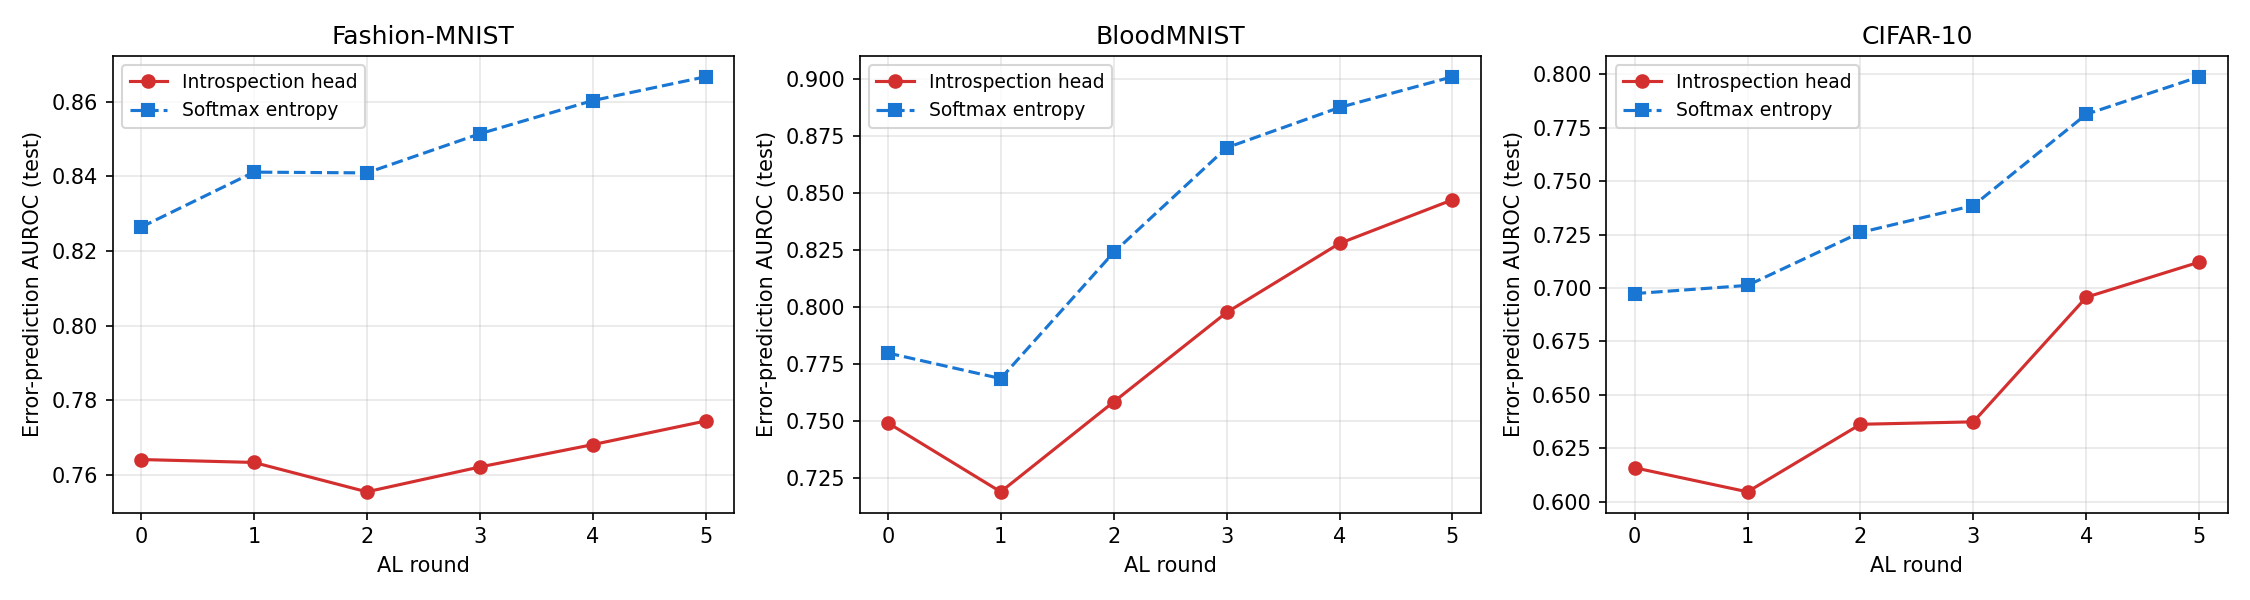
\includegraphics[width=\linewidth]{../results/diagnostics_auroc.png}}%
{\emph{[Diagnostics pending]}}
\caption{AUROC for error prediction on the test set: introspection head
versus softmax entropy, per AL round (perfect oracle), across all three
datasets. Entropy consistently ranks errors better --- yet wherever
selection is actually effective, it picks worse batches.}
\label{fig:auroc}
\end{figure}

\paragraph{Why it works: selection quality differs from error-ranking
quality.} A natural hypothesis is that \method{} succeeds because its
introspection head ranks model errors better than entropy does. The
evidence says otherwise --- a negative result that holds across all
three datasets. At distinguishing actual test errors, the introspection
score achieves an AUROC of \FmnistAurocIntro\% on Fashion-MNIST,
\BloodAurocIntro\% on BloodMNIST and \CifarAurocIntro\% on CIFAR-10 ---
figures that fall \emph{below} the corresponding softmax entropy scores
of \FmnistAurocEnt\%, \BloodAurocEnt\% and \CifarAurocEnt\%
(Figure~\ref{fig:auroc}) --- yet wherever selection proves effective,
entropy selects poor batches (Table~\ref{tab:main}). Entropy derives
its AUROC advantage from aleatorically ambiguous samples near the
decision boundary: prioritising them boosts AUROC cheaply, but as a
\emph{batch} they are highly redundant, and their labels are the least
reliable under a noisy oracle. The introspection head distributes its
mass differently --- trained on the history of model errors in feature
space rather than on instantaneous logit geometry --- and the
$k$-center gate transforms these comparatively weak point-wise signals
into robust batches. Batch selection quality therefore cannot be
reduced to point-wise error prediction; this distinction should be
measured rather than assumed when evaluating learned selection
functions.

\paragraph{Ablation.} Removing the diversity gate (\emph{\method{}
without diversity}) causes the perfect-oracle AUBC to drop on both
datasets: from \FmnistCleanIrisAubc\% to \FmnistCleanIrisNodivAubc\% on
Fashion-MNIST, and from \BloodCleanIrisAubc\% to
\BloodCleanIrisNodivAubc\% on BloodMNIST, where the final accuracy also
collapses from \BloodCleanIrisFinal\% to \BloodCleanIrisNodivFinal\%.
That drop on BloodMNIST --- the single largest ablation effect in this
study --- is the clearest evidence that iterative batch selection
driven directly by \emph{any} point-wise score (top-$K$) benefits from
the introspection head only when a diversity gate follows it. Removing
the reliability weight under noise (\emph{\method{} without
reliability}) causes the noisy-oracle final accuracy to fall from
\FmnistNoisyIrisFinal\% to \FmnistNoisyIrisNorelFinal\% on
Fashion-MNIST and from \BloodNoisyIrisFinal\% to
\BloodNoisyIrisNorelFinal\% on BloodMNIST (AUBC \BloodNoisyIrisAubc\%
$\to$ \BloodNoisyIrisNorelAubc\%); the ablated version still
outperforms most baselines by a small margin, implying that the
selection and label-acceptance components contribute additively rather
than redundantly. That additivity is what the BADGE experiment then
confirms from outside: the label-acceptance term keeps its value when
the selection term is replaced wholesale.

The same two ablations on CIFAR-10 say something different, and that
contrast is the point. There, dropping the reliability weight moves
nothing at all
(\CifarNoisyIrisNorelFinal\% versus \CifarNoisyIrisFinal\%,
$p=\CifarNoisyNorelPairedP$), whereas on the capable datasets it was worth up to
\FmnistNoisyIrisFinalGain{} points; the small-loss criterion needs a
model that has already learned something before it can tell a corrupted
label from a hard one, and below that threshold it does not so much
misfire as fall silent. Dropping the diversity gate still costs
accuracy (\CifarCleanIrisNodivFinal\% versus \CifarCleanIrisFinal\%),
so coverage remains useful regardless of model quality. Each component
therefore has its own precondition, and the capability gate of
Section~\ref{sec:application} is really a statement about the
introspection signal alone.

\section{Discussion}\label{sec:discussion}
\method{} operationalises --- \emph{inside} the classifier --- two
lessons that the applied HITL literature of 2026 keeps relearning at
the level of workflows: expert attention should be allocated to where
the model actually fails, and expert output should be treated with
scepticism. The mechanism is deliberately minimal --- a detached MLP
head, a greedy selection, and a loss reweighting --- so it integrates
easily with the expert-curation scheme of \citet{petso2026} (replacing
manual pool ordering), the annotation tooling of \citet{piccoli2026},
and deployment-time learning-to-defer \citep{mozannar2020,alves2025},
where the introspection score serves as a natural deferral signal.
Section~\ref{sec:application} details what that integration looks like
in a laboratory annotation pipeline and, equally importantly, what it
demands of managers: a batch size, an estimate of the annotator error
rate, and a capability check.

The results establish a practical threshold, with a dataset on either
side of it. Once the base model has sufficient capability, selection
--- whether learned or heuristic, as seen here on Fashion-MNIST and
BloodMNIST --- becomes beneficial, while the reliability gate
safeguards those gains against annotator errors. Of the two, the
Fashion-MNIST result is the one the seeds actually resolve; the
BloodMNIST result is the more interesting, since the method was not
tuned for that dataset at all, but at six seeds its margin stays inside
the noise and we treat it as corroboration rather than proof. In cold-start scenarios, such as training
CIFAR-10 from scratch with a few thousand labels, it is better to
allocate the initial portion of the budget to random sampling and leave
the \emph{selection} signal switched off until the model is good enough
for its own error predictions to mean something. Our cold-start
ablation is specific on this point: the reliability weight can be left
enabled, since it neither helps nor harms there, and the diversity gate
should be, since coverage still pays; it is introspection-driven
ranking that must wait. This leads to an immediate,
empirically testable next step: a warm-start strategy of initial random
or self-supervised sampling, followed by activation of
introspection-based selection and reliability weighting only once the
introspection head's validation AUROC crosses a threshold --- in
essence, the capability gate of Section~\ref{sec:application}.

BloodMNIST also sharpens a methodological question. Because every
point-wise-scored method starts behind random sampling but eventually
surpasses it, AUBC and final accuracy offer conflicting views of which
of those methods is best. Neither metric is incorrect; they simply
embody different stopping assumptions. A programme that deploys a model
only after exhausting the entire annotation budget should maximise the
endpoint value, whereas one that can halt as soon as accuracy is
sufficient should maximise the area under the curve. Papers that report
a single figure without specifying the underlying scenario are, on such
datasets, presenting a choice rather than a result.

\section{Limitations}\label{sec:limitations}
While symmetric label noise is common, it is the weakest noise model;
addressing instance-dependent and class-conditional annotator errors,
as documented by \citet{hussain2026} and \citet{alves2025}, remains
future work, as does the online estimation of $\gamma$, which we
assumed known following co-teaching \citep{han2018}. Our margin over
the best baseline is directionally consistent --- under the noisy
oracle, \method{} wins on \BloodNoisyIrisSeedsWon{} seeds for
BloodMNIST and \FmnistNoisyIrisSeedsWon{} seeds for Fashion-MNIST ---
but only the Fashion-MNIST difference exceeds the 5\% significance
level in paired tests ($p=\FmnistNoisyIrisPairedP$ versus
$p=\BloodNoisyIrisPairedP$); meanwhile, under the \emph{perfect}
oracle, \method{} is statistically indistinguishable from the best
baseline on both datasets ($p=\BloodCleanIrisPairedP$,
$p=\FmnistCleanIrisPairedP$). With six seeds, a margin well under a
point is hard to resolve, and we would rather report the BloodMNIST
result as an unconfirmed trend than lean on it. For CIFAR-10 there are
only \CifarNoisyNSeeds{} seeds, so the cold-start result rests on less
evidence still. To summarise honestly: the benefit under the noisy
oracle is established on one dataset, directionally supported on a
second, and absent in cold-start scenarios.

The budgets are also truncated. At 3,000 labels on BloodMNIST the
accuracy of every method is still rising, and \method{} exhibits the
steepest terminal slope under the noisy oracle; the observed ranking at
that point is therefore a snapshot of an unfinished curve --- a larger
budget could widen the gap or erase it, and we do not know which.
The experiments span three standard vision benchmarks at moderate
budgets; extending to ImageNet-scale pools and to text tasks, along
with direct comparisons against BADGE \citep{ash2020} and Learning-Loss
\citep{yoo2019}, would strengthen external validity. Finally, the human
element is synthetic; while BloodMNIST makes the \emph{data} medically
realistic, the annotator remains a symmetric-noise process rather than
a morphologist. The application logic of
Section~\ref{sec:application} is a design proposal, and a user study
with real annotators, comparable to that of \citet{petso2026}, is the
natural next step.

\section{Conclusion}\label{sec:conclusion}
A two-layer introspection head, a $k$-center diversity gate and a
low-loss reliability weight turn a standard classifier into a
noise-aware HITL learner, and separating them shows that the three are
not equally portable. The learned acquisition signal is a real
improvement on the prior learned signal, Learning-Loss, but it does not
overturn a well-built hybrid of uncertainty and diversity: BADGE
selects better batches than it does. The reliability weight is the part
that travels. It was designed alongside our selector and works just as
well bolted onto someone else's, which is the property that matters for
a mechanism intended to be adopted rather than merely reported. The effect
replicates on a medical dataset that received no hyperparameter tuning
at all, while the method's failure on CIFAR-10 delineates its scope:
use this approach only when the model already understands what it does
not know, and until then spend the initial labels at random. The
modification is architectural, cheap and drop-in; and the resulting
workflow requires no change in the annotator's behaviour --- they
simply continue doing what they were already doing, which is viewing an
image, assigning a label, and moving to the next one.

\clearpage
\section*{Declaration of competing interest}
The author declares no known competing financial interests or personal
relationships that could have appeared to influence the work reported
in this paper.

\section*{Data availability}
All three datasets are publicly available. Code, experiment logs and
the scripts that regenerate every number, table and figure in this
paper are released with the manuscript.

\printcredits

\bibliographystyle{cas-model2-names}
\bibliography{refs}

\end{document}
